\chapter{Las bases de las comunicaciones digitales basadas en la Radio Definida por Software}

%%%%%%%%%%%%%%%%%%%%%%%%%%%%%%%%%%%%%%%%%%%%%%%%%

\section{Modelo de capas}

%%%%%%%%%%%%%%%%%%%%%%%%%%%%%%%%%%%%%%%%%%%%%%%%%

\section{Los retos que impone la capa del mensaje}
\subsection{El Scrambiling}
La señal digital que proviene directamente del mensaje es aleatoria, pero no es de tipo gaussiano, ya que ciertas combinaciones de bits tienen más probabilidad de aparecer que otras, así por ejemplo es común observar largos chorros de 1s y de 0s. Lograr que la señal digital tenga una PSD plana, como la de una señal binaria aleatoria, con una sola muestra por bit, es importante para poder implementar con éxito las técnicas digitales para el uso óptimo del canal, pero también para aprovechar mejor el canal. 
Para realizar el Scrambling se utiliza una secuencia de pseudo ruido (PN, del inglés Pseudo Noise) (PRBS, es otra sigla usada para referirse a lo mismo, del inglés Pseudo Random Binary Sequence)\\

El scrambling puede ser representado por la interconexión que se presenta en la Fig.1, donde b(t) es el mensaje expresado en forma de señal binaria bipolar, c(t) es la secuencia PN, expresada también como señal binaria bipolar y bs(t) es la señal luego del scrambling. \\


%\setcounter{figure}{69}
\begin{figure}[h!]
	\captionsetup{justification = raggedright, singlelinecheck = false}
	\caption{Esquema de scrambling en forma de interconexión} 
	\centering
	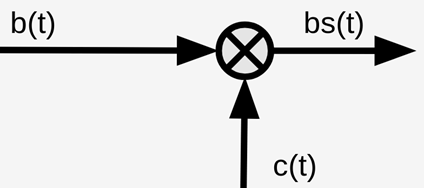
\includegraphics[scale=0.9]{Imagenes/Esquema.png}
	\label{fig:Esquema}
%	\captionsetup{justification=raggedright,font={scriptsize,bf,it}}
%	\caption*{fuente: Tomado del libro de Haykin}
\end{figure}

En la \textcolor{Red}{Fig. 3} se presenta un ejemplo de scrambling, cuando la secuencia PN es 0010100010 y el mensaje es 1000111010, entonces la señal aleatorizada es 010110011. 


\vspace{200px}
\begin{figure}[h!]
	\captionsetup{justification = raggedright, singlelinecheck = false}
	\caption{Ejemplo de scrambling} 
	\centering
	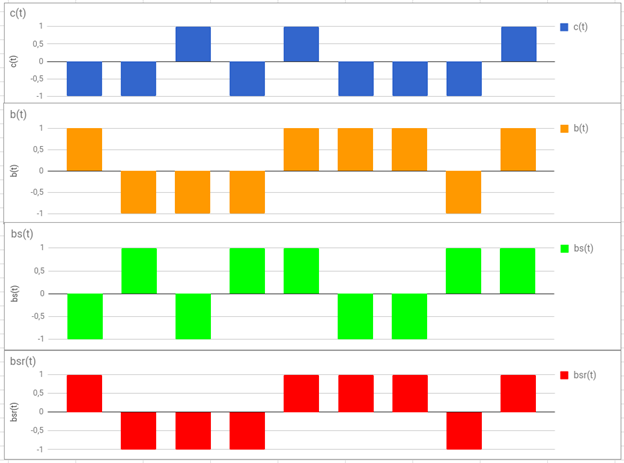
\includegraphics[scale=0.9]{Imagenes/scrambling.png}
	\label{fig:scrambling}
	%	\captionsetup{justification=raggedright,font={scriptsize,bf,it}}
	%	\caption*{fuente: Tomado del libro de Haykin}
\end{figure}

De igual manera es posible demostrar que el esquema de la Fig.1, puede usarse también para el de-scrambling, para ello se usa la señal bs(t) como entrada, el mismo código PN usado en el scrambling y se obtiene bsr(t) como salida que es la misma señal b(t).\\

De este ejemplo se deduce también que la señal que resulta del scrambling hereda la aleatoriedad que tiene la secuencia PN, con lo cual se logra el objetivo de hacer que la PSD de la señal que se obtiene sea la que corresponde a una señal binaria aleatoria bipolar.

%%%%%%%%%%%%%%%%%%%%%%%%%%%%%%%%%%%%%%%%%%%%%%%%%

\section{La modulación Digital Bandabase}

Este capítulo explica la modulación digital paso bandas desde un enfoque poco común en la literatura, pero muy necesario para el estado tecnológico de hoy. Se enfoca en los conocimientos necesarios para poder llegar a realizar una implementación basada en Software Defined Radio con un equipo como el USRP que permite realizar una transmisión real. \\
\begin{itemize}
	\item [$\bullet$] La señal paso bandas es una onda senoidal de frecuencia fc que lleva la información codificada ya sea en la fase, en la amplitud, en la frecuencia, o en en una combinación de esos parámetros, los cuales consecuentemente varía en el tiempo. 
	 \begin{equation} \label{capcuatro_uno}
	 	 y(t) = B(t)cos(2 \pi [f_c+f(t)]t+ \varphi t)
     \end{equation}
	
	\item [$\bullet$] Los sistemas de comunicaciones modernos , como las comunicaciones móviles 4G o los enrutadores WiFi no usan una sola modulación, como en los tiempos de antes. Más bien escogen de manera inteligente la modulación que mejor se adapta a las condiciones del canal en el momento. Además usan mayormente la fase y la amplitud de la portadora, lo cual se puede representar así:

 \begin{equation} \label{capcuatro_dos}
	  y(t)=B(t)cos[2 \pi f_ct + \varphi(t)] 
 \end{equation}

	
	\item [$\bullet$] Como ya se ha visto, si este concepto se lleva a SDR con USRP, la señal paso bandas anteriormente descrita es la que entrega el USRP, mientras que la programación en SDR debe enfocarse en producir la señal que se le debe entregar al USRP que no es otra cosa que la Envolvente Compleja $y_CE(t)$ de $y(t)$. Eso significa que programar una modulación en SDR para un sistema de comunicación real es programar la versión banda base de esa modulación paso bandas, que no es otra cosa que la Envolvente Compleja. 

 \begin{equation} \label{capcuatro_tres}
	 y_{CE}(t)=2B(t)e^{j\varphi(t)}
 \end{equation}

	\item [$\bullet$] Desde este punto de vista, el mensaje no modula parámetros de una portadora senoidal, sino de una señal exponencial compleja. También podemos decir que lo que se modula es una portadora en versión banda base o en versión de envolvente compleja.
	
	\item [$\bullet$] En los métodos de modulación más básicos, estos parámetros cambian cada vez que cambia el código o clave que debe llevar.
	
	\item [$\bullet$] La regla que define como cambian los parámetros de la señal exponencial compleja puede ser expresada por medio de una tabla que es comúnmente conocida como tabla de verdad o mediante un diagrama de constelaciones.
	
		\begin{table}[h!]
		\captionsetup{justification = raggedright,singlelinecheck = false}
		\caption{\label{tabla:tabla2} Plantilla para la Tabla de Verdad}
		\begin{center}
			\scalebox{0.75}{
				\begin{tabular}{|l|l|l|}
					\hline
					\multicolumn{2}{|c|}{\textbf{TABLA DE VERDAD}}\\ \hline
					La clave & Lo que la clave modifica en la portadora o el  \\ \hline
					& valor que toma la señal exponencial compleja \\ \hline
					&  \\ \hline
					&  \\ \hline
			\end{tabular}}
		\end{center}
	\end{table}

	\item [$\bullet$] Esto se explica mejor con ejemplos que se ilustran en los siguientes capítulos.

\end{itemize}

%%%%%%%%%%%%%%%%%%%%%%%%%%%%%%%%%%%%%%%%%%%%%%%%%%%

\section{La modulación BPSK}
Esta modulación se distingue porque:

\begin{itemize}
	\item [$\bullet$] El mensaje es de tipo: binario, de modo que el código o clave que puede modificar los parámetros de la portadora puede tomar el valor 1 o el 0
	\item [$\bullet$] El parámetro de la portadora que es modificado es: la fase. Consecuentemente solo se tienen dos posibles estados para la fase. Usualmente la fase toma los valores 0 y $\pi$, pero también es BPSK si toma los valores $-\pi/2$ y $\pi/2$ o cualquier otros dos valores separados entre sí en un ángulo $\pi$ 
	\item [$\bullet$] Para generar la envolvente compleja lo usual es considerar que la fase pueda tomar los valores 0 y , por lo tanto, la Envolvente compleja está dada por:
	
 \begin{equation} \label{capcuatro_cuatro}
			 y_{CE}(t) = y_{I}(t) +j y_{Q}(t), donde  \begin{cases}  y_{I}(t) = Ae^{j0}, cuando- entra- un -0\\ y_{Q}(t) = Ae^{j\pi}, cuando- entra- un -1
			\end{cases}
\end{equation}

 \begin{equation} \label{capcuatro_cinco}
	O donde  \begin{cases}  y_{I}(t) = A, cuando / entra / un -0\\ y_{Q}(t) = -A, / cuando / entra / un  / -1
	\end{cases}
\end{equation}

Donde A es la magnitud de los símbolos que son entregados al USRP.
	\item [$\bullet$] La tabla de verdad resume lo anterior así:
	
			\begin{table}[h!]
		\captionsetup{justification = raggedright,singlelinecheck = false}
		\caption{\label{tabla:tabla3} Tabla de Verdad de la Modulación BPSK en Función de la Fase}
		\begin{center}
			\scalebox{0.75}{
				\begin{tabular}{|l|l|l|}
					\hline
					\multicolumn{2}{|c|}{\textbf{TABLA DE VERDAD DE LA MODULACIÓN BPSK}}\\ \hline
					Clave & Fase  \\ \hline
				0	& 0\\ \hline
				1	& $\pi$ \\ \hline
			%		&  \\ \hline
			\end{tabular}}
		\end{center}
	\end{table}
Otra manera de decir lo mismo es la siguiente.
%\vspace{200px}
			\begin{table}[h!]
	\captionsetup{justification = raggedright,singlelinecheck = false}
	\caption{\label{tabla:tabla4} Tabla de Verdad de la Modulación BPSK en Función de la Amplitud Compleja}
	\begin{center}
		\scalebox{0.75}{
			\begin{tabular}{|l|l|l|}
				\hline
				\multicolumn{2}{|c|}{\textbf{TABLA DE VERDAD DE LA MODULACIÓN BPSK}}\\ \hline
				Clave & Fase  \\ \hline
				0	& $Ae^{j0}$\\ \hline
				1	& $Ae^{j\pi}$ \\ \hline
				%		&  \\ \hline
		\end{tabular}}
	\end{center}
\end{table}

o la siguiente. \\

			\begin{table}[h!]
	\captionsetup{justification = raggedright,singlelinecheck = false}
	\caption{\label{tabla:tabla5} Tabla de Verdad de la Modulación BPSK en Función de la amplitud}
	\begin{center}
		\scalebox{0.75}{
			\begin{tabular}{|l|l|l|}
				\hline
				\multicolumn{2}{|c|}{\textbf{TABLA DE VERDAD DE LA MODULACIÓN BPSK}}\\ \hline
				Clave & Fase  \\ \hline
				0	& $A$\\ \hline
				1	& $-A$ \\ \hline
				%		&  \\ \hline
		\end{tabular}}
	\end{center}
\end{table}
\end{itemize}
O en un diagrama polar, conocido como diagrama de constelaciones.

%\setcounter{figure}{78}
\begin{figure}[h!]
	\captionsetup{justification = raggedright, singlelinecheck = false}
	\caption{Diagrama de constelaciones BPSK}
	\centering
	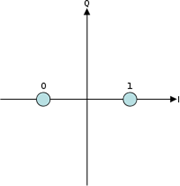
\includegraphics[scale=1]{Imagenes/Constelaciones.png}
	\label{fig:Constelaciones}
%	\captionsetup{justification=raggedright,font={scriptsize,bf,it}}
%	\caption*{fuente: \textcolor{
%			Orange}{Tomada de Wikipedia}}
\end{figure}

La señal paso bandas, a la salida del upconverter se puede deducir por su paso por el siguiente esquema:

\vspace{300px}
\begin{figure}[h!]
	\captionsetup{justification = raggedright, singlelinecheck = false}
	\caption{Esquema señal paso banda}
	\centering
	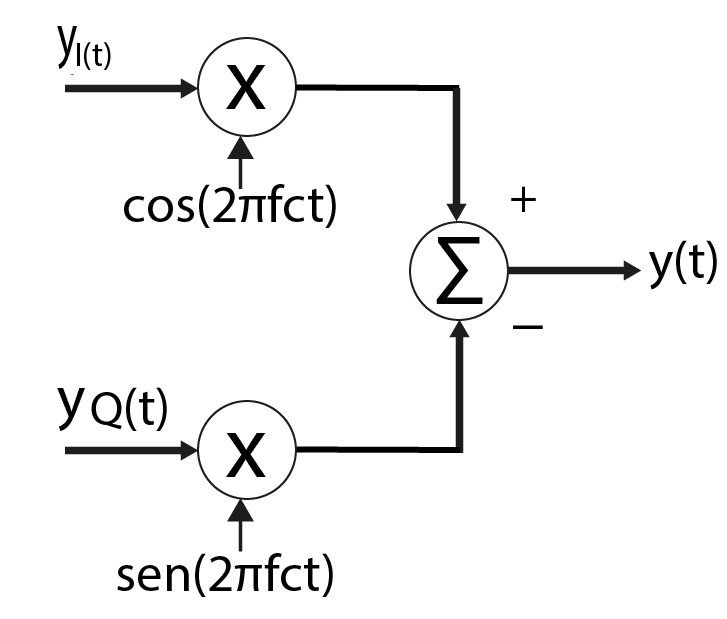
\includegraphics[scale=0.3]{Imagenes/Y.png}
	\label{fig:Y}
	%	\captionsetup{justification=raggedright,font={scriptsize,bf,it}}
	%	\caption*{fuente: \textcolor{
	%			Orange}{Tomada de Wikipedia}}
\end{figure}		

La calidad de la señal enviada, respecto al ruido del canal está en función de la amplitud D de la señal s(t) que entrega el USRP el cual tiene varios elementos que alteran la amplitud como filtros y amplificadores:

 \begin{equation} \label{capcuatro_seis}
	  s(t)=D cos[2\pi f_{c}t+\varphi(t)] donde \varphi(t) = \begin{cases} 0, cuando- entra- un -0\\ \pi, cuando- entra- un -1 
	\end{cases}
\end{equation}

Donde $D=AK_a$ y $K_a$ representa la amplificación total que aplica el USRP. \\

Para llegar a conocer el desempeño de esta modulación ante el ruido, es necesario formular esta expresión en términos de la energía $E_s$ que lleva cada símbolo, la cual para el caso de la BPSK es lo mismo que la energía $E_b$ que lleva cada bit, pues cada símbolo contiene solo un bit en el caso de la BPSK. Esa energía es igual a la potencia promedio de la señal multiplicada por la duración del bit.\\

 \begin{equation} \label{capcuatro_siete}
	 E_b=PT_{b}
\end{equation}

A su vez, sabemos que:

 \begin{equation} \label{capcuatro_ocho}
	 V_{RMS}=\frac{D\sqrt{2}}{2}
\end{equation}

Por lo tanto, la energía contenida en cada bit, en la señal modulada paso bandas, es en promedio:

 \begin{equation} \label{capcuatro_nueve}
	 E_{b}=\frac{D^{2}T_b}{2}
\end{equation}

De aquí, que.

\begin{equation} \label{capcuatro_diez}
	 D=\sqrt{\dfrac{2E_b}{T_b}}
\end{equation}

Para obtener finalmente que:

\begin{equation} \label{capcuatro_once}
	 s(t)= \sqrt{\dfrac{2E_{b}}{T_{b}}} \cos [2\pi f_{c}t+\varphi(t)] donde \varphi(t)= \begin{cases} 0, cuando- entra- un -0\\ \pi, cuando- entra- un -1 
	\end{cases}
\end{equation}

De modo que cuando la señal pasobandas está antes de la antena transmisora del USRP se puede expresar como: 

\begin{equation} \label{capcuatro_doce}
	 s(t)= K_aA\cos [2\pi f_ct+\varphi(t)] donde \varphi(t)= \begin{cases} 0, cuando- entra- un -0\\ \pi, cuando- entra- un -1 
	\end{cases}
\end{equation}

Pero, más allá de la antena, el parámetros $E_b$ se desvanece por el efecto de la propagación y aparece una componente adicional el ruido. \\

Veamos el siguiente ejemplo. Se tiene una  información binaria aleatoria y debe ser enviada a un lugar distante por un medio inalámbrico. La señal de voltaje que se le entrega a la antena transmisora debe ser una senoidal con frecuencia $f_c$, de modo que pueda ser traducida a una onda electromagnética que puede atravesar la distancia hasta llegar al receptor. \\

\begin{figure}[h!]
	\captionsetup{justification = raggedright, singlelinecheck = false}
	\caption{Formación de la señal BPSK} 
	\centering
	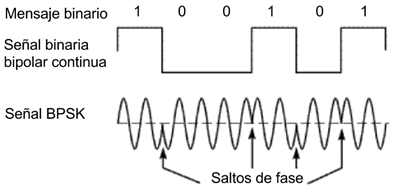
\includegraphics[scale=1]{Imagenes/BPSK-1.png}
	\label{fig:BPSK-1}
	%	\captionsetup{justification=raggedright,font={scriptsize,bf,it}}
	%	\caption*{fuente: \textcolor{
	%			Orange}{Tomada de Wikipedia}}
\end{figure}

La figura \ref{fig:BPSK-1} ilustra las modificaciones de fase que una clave binaria (un uno o un cero) introduce en la portadora para que ese mensaje pueda cruzar la distancia en forma de una onda que va sufriendo saltos de fase. \\

Para realizar un montaje real, usando GNU radio y un USRP es necesario tener en cuenta las siguientes consideraciones: \\

\begin{itemize}
	\item [$\bullet$] La señal senoidal de la figura 1, estará a la salida del USRP. Esa señal usualmente no será vista por el programador de GNU, ni siquiera usando un osciloscopio físico conectado a la salida del USRP por dos razones: 
	\begin{itemize}
		\item [$\bullet$] Porque la portadora tiene, en la práctica, una frecuencia demasiado alta, lo cual hace difícil de apreciar los saltos de fase;
		
		\item [$\bullet$] El ancho de banda de la señal física es acotado, mientras que la teórica es infinito, por eso en la primera no se apreciaran los bruscos saltos de frecuencia que se aprecian en la segunda. Así por ejemplo, los moduladores que trae la biblioteca de GNU radio llevan implícitamente un filtro coseno alzado con un factor de rolloff que el programador puede elegir entre 0 y 1.
	\end{itemize}
	\item [$\bullet$] El programador debe conocer la forma de la señal que debe ser entregada al USRP, que, como ya se vió, es la envolvente compleja de la señal que produce el USRP. 
\end{itemize}

\subsection{La Envolvente compleja}

\subsection{La tabla de verdad}
\subsection{La constelación}

%%%%%%%%%%%%%%%%%%%%%%%%%%%%%%%%%%%%%%%%%%%%%%%%%%

\section{Retos que impone el ancho del banda del canal}
\subsection{Generalidades sobre la Forma de los pulsos en tiempo}
Supongamos que se tiene una computadora y esta debe enviar información binaria hacia otra computadora mediante un cable de cobre. El cable es un canal capaz sólo de conducir señales eléctricas. El proceso de convertir la información binaria en pulsos eléctricos es lo que llamamos Formación de pulsos o en inglés Wave Forming. 

%\setcounter{figure}{53}
\begin{figure}[h!]
	\captionsetup{justification = raggedright, singlelinecheck = false}
	\caption{La necesidad de pulsos continuos en una comunicación de datos discretos} 
	\centering
	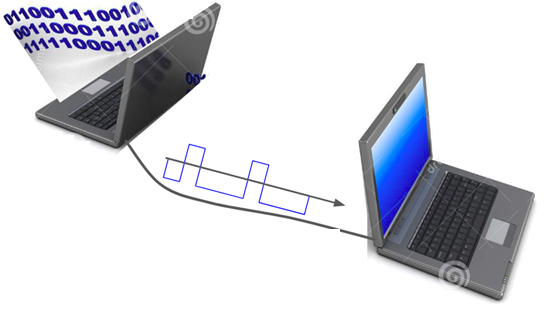
\includegraphics[scale=0.7]{Imagenes/Computador.png}
	\label{fig:Computador}
	%	\captionsetup{justification=raggedright,font={scriptsize,bf,it}}
	%	\caption*{fuente: llllll}
\end{figure}

Pueden haber varias causas para darle forma a los pulsos, pero lo esencial consiste en la  necesidad de adaptar la señal a las condiciones que impone el canal. En este sentido, sobre un cable las señales viajan como pulsos eléctricos limitados a las condiciones del cable, pero ellas también pueden viajar sobre un canal inalámbrico, lo cual implica hacerlo en forma de ondas electromagnéticas, en una banda limitada en ancho de banda y centrada en la frecuencia de la portadora. En el segundo caso, si se usan técnicas de SDR, el Up-converter y la antena realizan gran parte del trabajo, pero debemos entonces entregar las formas de onda apropiadas al Up-converter para que este realice su trabajo,

Lo primero que se nos ocurre es que estos pulsos tengan forma rectangular, pero en realidad nada impide que puedan tener cualquier otra forma. Lo cierto es que la forma que se elija tiene varias implicaciones.\\

A continuación se brinda una solución teórica, en el dominio de tiempo continuo, pero que da claras luces para una implementación práctica. La idea consiste en contar con un sistema lineal e invariante en el tiempo (LIT) con una respuesta al impulso $h(t)$ que tenga la forma del pulso deseado. Para que la idea funcione es necesario convertir de alguna manera la información binaria a una señal digital en impulsos tipo $A \delta (t)$, donde $A=1$ para los 1 y $A=-1$ para los ceros, como se muestra en la Figura  \ref{fig:Secuencia1} para un  ejemplo donde los datos son 1 0 1 1 0 1 0 y la forma de onda deseada es rectangular.
\begin{figure}[h!]
	\captionsetup{justification = raggedright, singlelinecheck = false}
	\caption{Formador de pulsos rectangulares implementado mediante un Sistema LIT} 
	\centering
	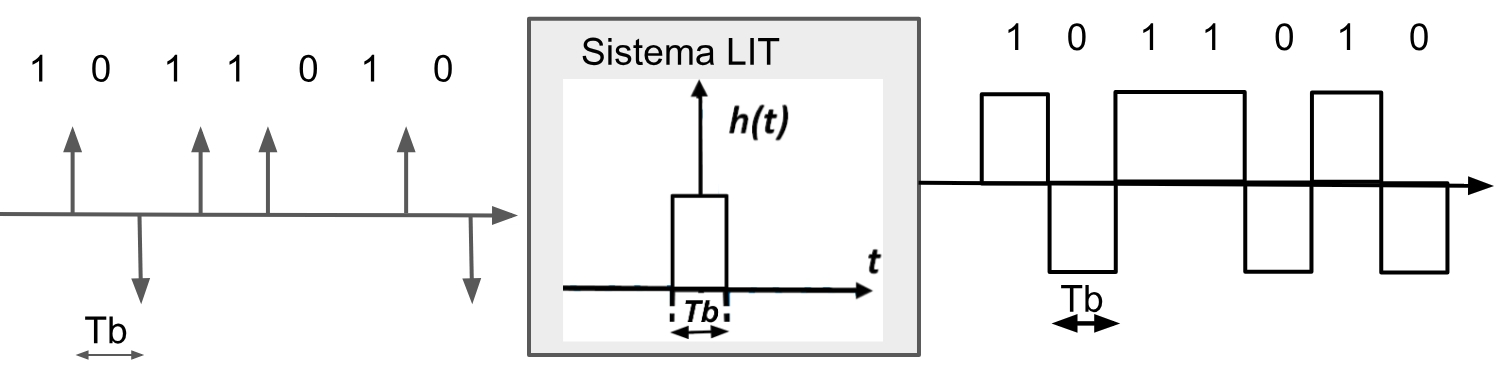
\includegraphics[scale=0.3]{Imagenes/waveform_rect.jpg}
	\label{fig:Secuencia1}
	%	\captionsetup{justification=raggedright,font={scriptsize,bf,it}}
	%	\caption*{fuente: Tomado de Haykin}
\end{figure}

En el dominio discreto, la realización es muy similar [\textcolor{red}{falta}]

\subsection{La Interferencia Intersimbolo debido a la forma de los pulsos}

Las señales de forma rectangular tienen la desvenja de ocupar un gran ancho de banda, pero tratar de limitar eses ancho de banda usando señales con otras formas diferentes puede traducirse en un problema conocido como Interferencia Intersímbolo (ISI). En la Figura \ref{fig:Intervalos} se muestra un ejemplo de lo significaría hacer pasar una señal binaria con formas rectangulares por un filtro que restrija notablemente el ancho de banda. Podemos apreciar como la energía de un bit afecta al bit vecino. En la parte receptora, para intentar recuperar los bits, es posible muestrear la señal recibida en los intervalos de muestreo que presenta la figura \ref{fig:Intervalos} para obtener la mejor aproximación de la señal original y poder regenerar los bits, por ejemplo comparando cada muestra con el nivel de amplitud cero, osea que si la muestra tiene un valor mayor a cero es un uno, de lo contrario es un cero. Sin embargo, observamos que se pueden presentar errores, los cuales pueden agravarse aún más ante la presencia de ruido y distorsiones propias de un canal real. \\

%\vspace{200px}
\begin{figure}[h!]
	\captionsetup{justification = raggedright, singlelinecheck = false}
	\caption{Comparación de una señal aleatoria bipolar de forma ideal con la forma que puede tomar al acotar su ancho de banda} 	\centering
	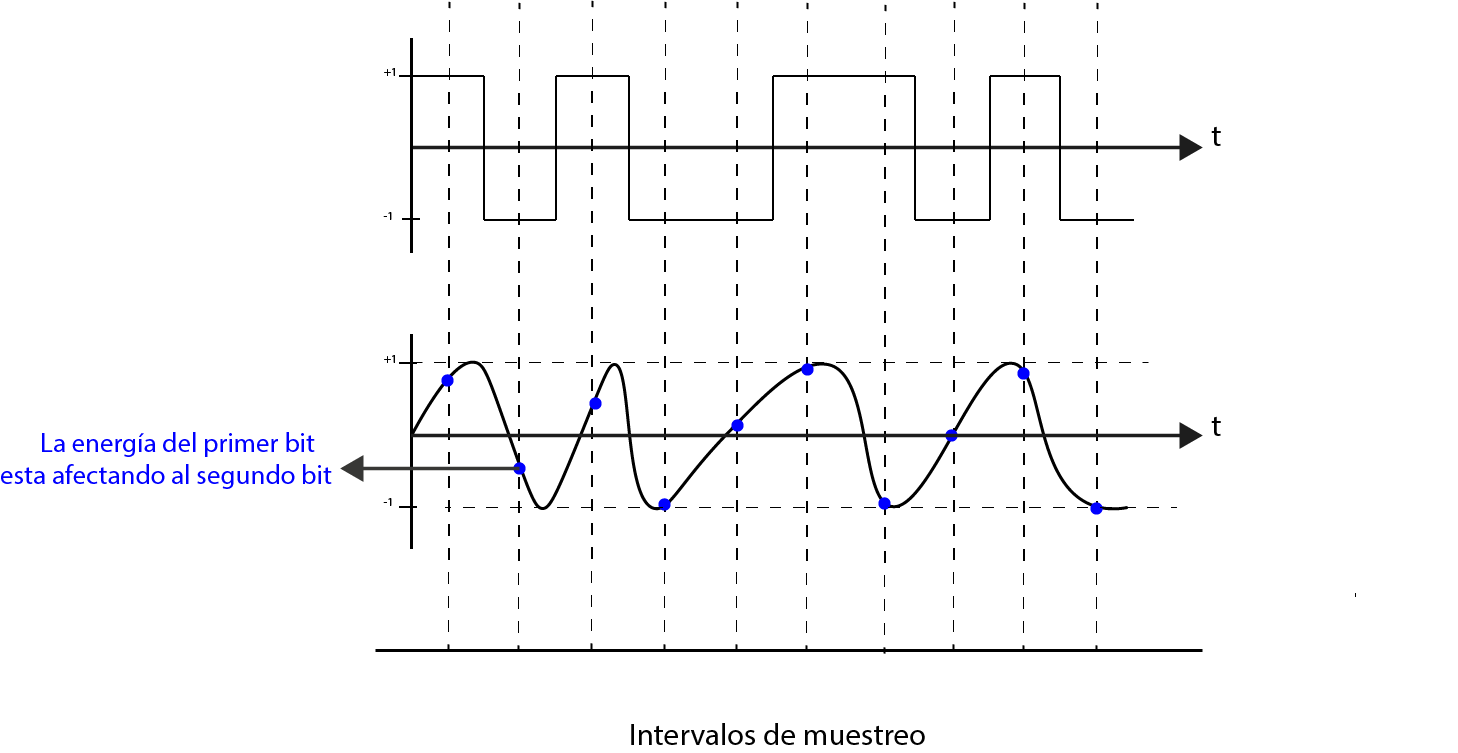
\includegraphics[scale=0.3]{Imagenes/Intervalos.png}
	\label{fig:Intervalos}
	%	\captionsetup{justification=raggedright,font={scriptsize,bf,it}}
	%	\caption*{fuente: Tomado de Haykin}
\end{figure}

\subsection{Diagrama de Ojo}
Podríamos decir que se trata de una herramienta de visualización de las señales digitales, especialmente las binarias. En la página web del libro se tiene un vídeo sobre ClearCurve que explica muy bien lo que significa el diagrama de Ojo. El enlace es el siguiente

\begin{center}
\url{https://sites.google.com/saber.uis.edu.co/comdig/m/wf} 
\end{center}
La figura \ref{fig:Ojo} explica las partes del ojo.

\begin{figure}[h!]
	\captionsetup{justification = raggedright, singlelinecheck = false}
	\caption{Diagrama de Ojo.} 
	\centering
	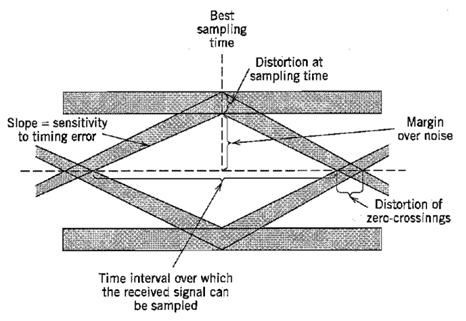
\includegraphics[scale=0.8]{Imagenes/Ojo.png}
	\label{fig:Ojo}
		\captionsetup{justification=raggedright,font={scriptsize,bf,it}}
		\caption*{fuente: Tomado del Libro de Haykin}
\end{figure}


\subsection{Forma de pulsos basada en de Criterio de Nyquist}

La forma de la transformada de Fourier de un un pulso analítico o teórico, guarda relación con la forma de la PSD de una señal digital aleatoria representada por esos mismos pulsos. Por ejemplo, si se tiene una señal rectangular y se conoce la TF, entonces cuando se tiene una señal digital aleatoria, expresada por pulsos rectangulares aleatorios, la PSD también va a tener la una forma parecida a la TF de un pulso rectangular.\\
La Tabla \ref{tabla:tabla1} ha sido preparada para comprender mejor lo anterior. En la parte superior de la tabla se presenta la forma de pulso más conocida, se trata del pulso rectangular. También se presenta allí su forma equivalente en el dominio de las frecuencias de acuerdo a la Transformada de Fourier. Los siguientes son los detalles a destacar:

\begin{itemize}
    \item [$\bullet$] En el dominio del tiempo la señal es rectangular y está acodada a la duración $T_b$ seg. En el dominio de las frecuencias en cambio, tiene forma de función sinc y tiene un ancho de banda infinito.
    \item [$\bullet$] Por lo anterior, este pulso tiene un ancho de banda infinito
    \item El espectro pasa por cero en las que son múltiplo entero de $R_b=\frac{1}{T_b}$. En otras palabras, el espectro tiene lóbulos de duración $R_b$, pero en el centro el lóbulo es de doble duración, lo que equivale a considerar que allí hay dos lóbulos seguidos.
    \item [$\bullet$]  Si el impulso en el tiempo tiene amplitud $A$ y duración $T_b$, el espectro tiene una amplitud igual a $A \cdot_b$
\end{itemize}

\vspace{300px}
\begin{table}[h!]
	\captionsetup{justification = raggedright,singlelinecheck = false}
	\caption{\label{tabla:tabla6} Paralelo entre TF pulsos y PSD de pulsos aleatorios}
    \begin{center}
        \begin{tabular}{|l|}
        \hline
        \textbf{Transformada de Fourier de una señal analítica x(t)} \\
        \hline 
        \\  \hspace{13mm} 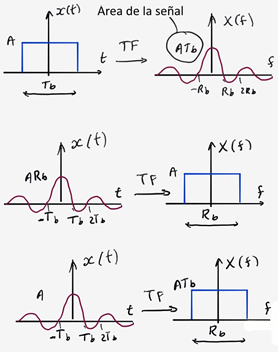
\includegraphics[scale=1]{Imagenes/Transfor.png}\\
        \hline
        \textbf{PDS de una señal de pulsos aleatoria}\\
        \hline
        \\ \hspace{13mm} 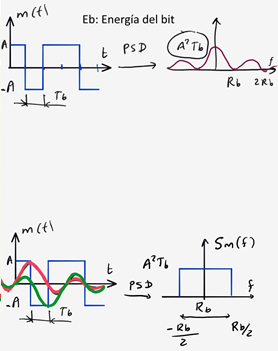
\includegraphics[scale=1]{Imagenes/Energia.png}\\
        \hline

        \end{tabular}
    \end{center}
\end{table}

En la misma Tabla \ref{tabla:tabla1}, debajo del pulso rectangular se tiene el caso contrario, donde la señal que en el tiempo tiene forma de función sinc, de duración infinita y con amplitud igual a $A R_b$. Entonces, por la propiedad de Dualidad de la Transformada de Fourier, se tiene que la TF es una pulso cuadrado en el dominio de las frecuencias, de altura A y un ancho de banda acotado, ya que ese pulso tiene un ancho igual a $R_b$. 

Pero las señales anteriores son determinísticas. En la práctica, sobre todo en las comunicaciones las señales que llevan información son aleatorias. En la segunda parte de la Tabla \ref{tabla:tabla1} se tiene dos casos equivalentes a los vistos anteriormente. En primer lugar vemos una señal aleatoria de pulsos rectangulares, pero aleatoria. Como estamos tratando con señales aleatorias, ya no podemos hablar de TF sino de PSD. Pero casualmente, la PSD de esta señal coincide en forma con la TF de un pulso determinístico, pero la altura ahora $A^2 T_b$. 
De manera similar, como se muestra más abajo, es posible generar una señal binaria con pulsos aleatorios con forma sinc y en este caso, la PSD tiene forma rectangular.

Lo más destacable de este razonamiento es lo siguiente:
\begin{itemize}
\item [$\bullet$] Existe una relación entre la TF de una señal determinística y la PSD de una señal donde esa señal determinística aparece aleatoriamente en un secuencia determinada.
\end{itemize}


Sabemos que la PSD de una señal binaria bipolar con rata de bits $R_b=\frac{1}{T_b}$ tiene la forma de la función sinc(.) al cuadrado, que se presenta en la Figura \ref{fig:PSD-ejemplo}. \\

% \vspace{200px}
%\setcounter{figure}{67}
\begin{figure}[h!]
	\captionsetup{justification = raggedright, singlelinecheck = false}
	\caption{PSD de una señal binaria aleatoria bipolar con pulso de duración $T_b$} 
	\centering
	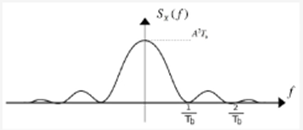
\includegraphics[scale=1]{Imagenes/PSD-ejemplo.png}
	\label{fig:PSD-ejemplo}
	%	\captionsetup{justification=raggedright,font={scriptsize,bf,it}}
	%	\caption*{fuente: Tomado de Haykin}
\end{figure}

Lo primero que salta a la vista es que su transmisión requiere un ancho de banda infinito. Eso significaría, por ejemplo, que una persona con un teléfono celular debería ocupar todo el espectro electromagnético para emitir señales digitales. Una opción para seguir usando este tipo de señales consiste en hacerla pasar previamente por un filtro que acote su ancho de banda para ajustarse al ancho de banda del canal. Aunque esto no resulta en una señal idealmente rectangular, es posible reconocerla en el receptor y recuperar la información en ella contenida. Podríamos decir que esto es gracias a que gran parte de la energía de la señal está contenida en las frecuencias bajas. 

Luego, de lo visto en el punto anterior surge una gran pregunta: ¿Cuál es el menor ancho de banda que puede llegar soportar una señal binaria aleatoria bipolar sin que esta se vea afectada por ISI? \\

La respuesta a esta pregunta se puede formular de la siguiente manera: La Figura \ref{fig:Solucion} muestra la forma de la señal acotada en ancho de banda, pero que está libre de ISI en ciertos instantes de tiempo que pueden ser elegidos en el receptor como los instantes más apropiados para realizar el muestreo.

\vspace{400px}
\begin{figure}[h!]
	\captionsetup{justification = raggedright, singlelinecheck = false}
	\caption{Comparación de una señal aleatoria bipolar de forma ideal con la forma que puede tomar al acotar su ancho de banda, de manera que quede libre de ISI en algunos instantes} 
	\centering
	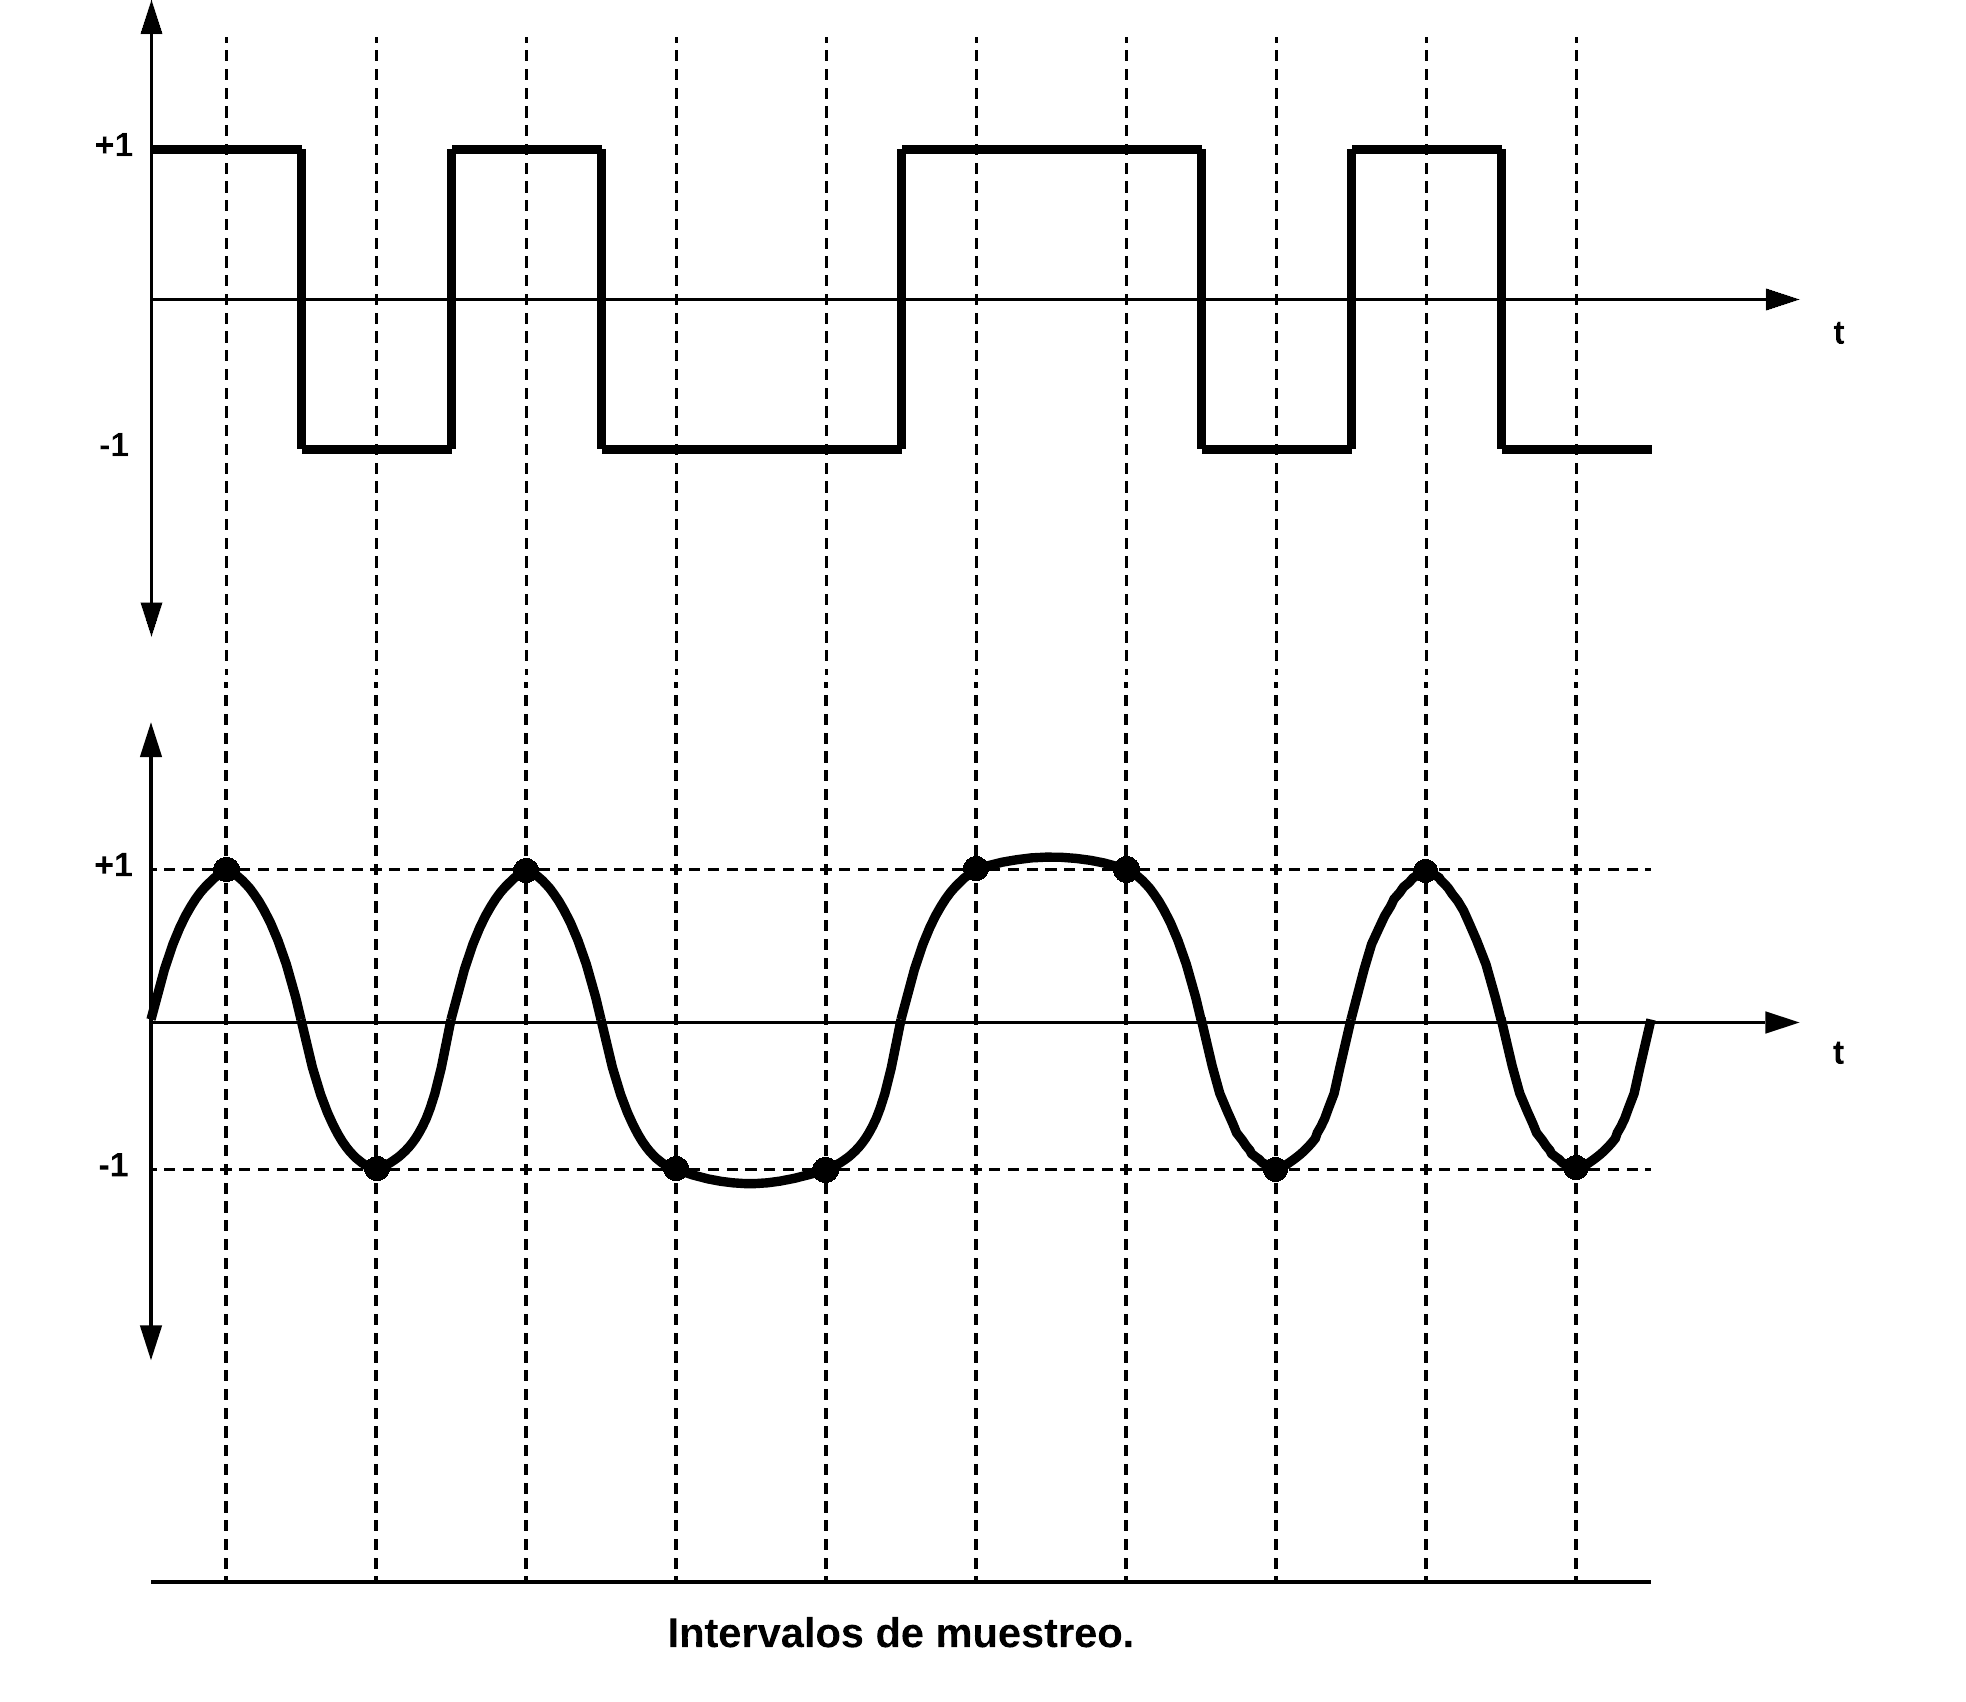
\includegraphics[scale=0.3]{Imagenes/Solucion.png}
	\label{fig:Solucion}
	%	\captionsetup{justification=raggedright,font={scriptsize,bf,it}}
	%	\caption*{fuente: Tomado de Haykin}
\end{figure}

Está demostrado \footnote{Simon Haykin [17], 2001 pág 261-267} que cada bit debería tomar la forma de una función sinc() para lograr dos cosas: evitar la ISI en el instante de muestreo; reducir al máximo el ancho de banda. \\

\begin{figure}[h!]
	\captionsetup{justification = raggedright, singlelinecheck = false}
	\caption{Filtro de Nyquist.} 
	\centering
	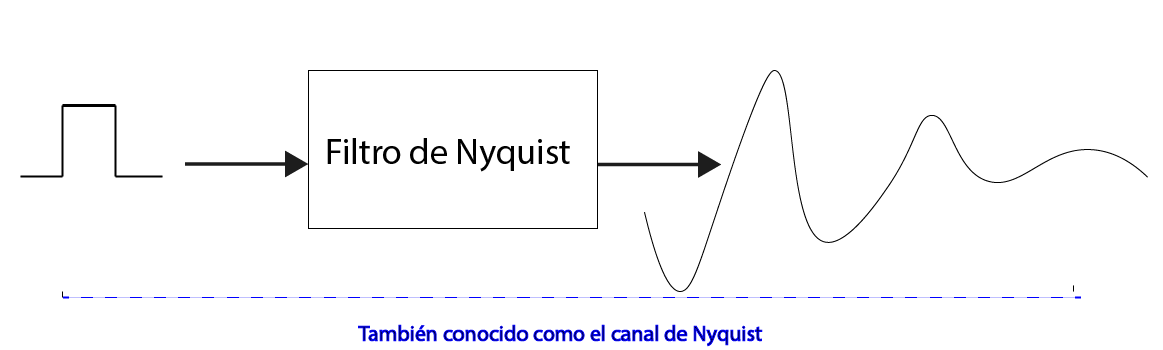
\includegraphics[scale=0.4]{Imagenes/Canal.png}
	\label{fig:Canal}
	%	\captionsetup{justification=raggedright,font={scriptsize,bf,it}}
	%	\caption*{fuente: Tomado de Haykin}
\end{figure}

De modo que si tomamos como ejemplo la secuencia binaria: 1011010. La forma de la señal en el tiempo será como la de la Figura \ref{fig:Secuencia}.\\

\subsection{Implementación del criterio de Nyquist}
\subsubsection{Implementación en forma continua}
El Filtro de Nyquist puede ser visto como el sistema que ante una entrada en forma de pulso rectangular responder con una salida en forma de función sinc. A continuación se brinda una solución teórica, en el dominio de tiempo continuo, pero que da claras luces para una implementación práctica en el dominio de tiempo discreto. La idea consiste en contar con un sistema lineal e invariante en el tiempo (LIT) con una respuesta al impulso $h(t) = sinc(\dfrac{t}{T_{b}})$. Para que la idea funcione es necesario convertir de alguna manera los pulsos rectangulares conrrespondientes a la señal digital en impulsos tipo $A \delta (t)$, donde $A=1$ para los 1 y $A=-1$ para los ceros. En la Figura  \ref{fig:Secuencia} se presenta un ejemplo para el caso en que la señal digital es binaria corresponde a los datos 1 0 1 1 0 1 0. Cabe aclarar que la señal de salida en la Figura  \ref{fig:Secuencia} se ha realizado con propósitos pedagógicos para mostrar como se superponen los diferentes pulsos que se van generando a la salida del sistema LIT, está claro que en la práctica lo que aparece es una sola señal que es la suma de todos los pulsos. Lo importante es lograr que en la señal de salida, cada Tb se logre identificar el valor de un bit gracias a que hay un instante en la duración de ese bit en que no está interferido por las señales que corresponden a los demás bits.\\

% \vspace{200px}
\begin{figure}[h!]
	\captionsetup{justification = raggedright, singlelinecheck = false}
	\caption{El Filtro de Nyquist implementado mediante un Sistema LIT} 
	\centering
	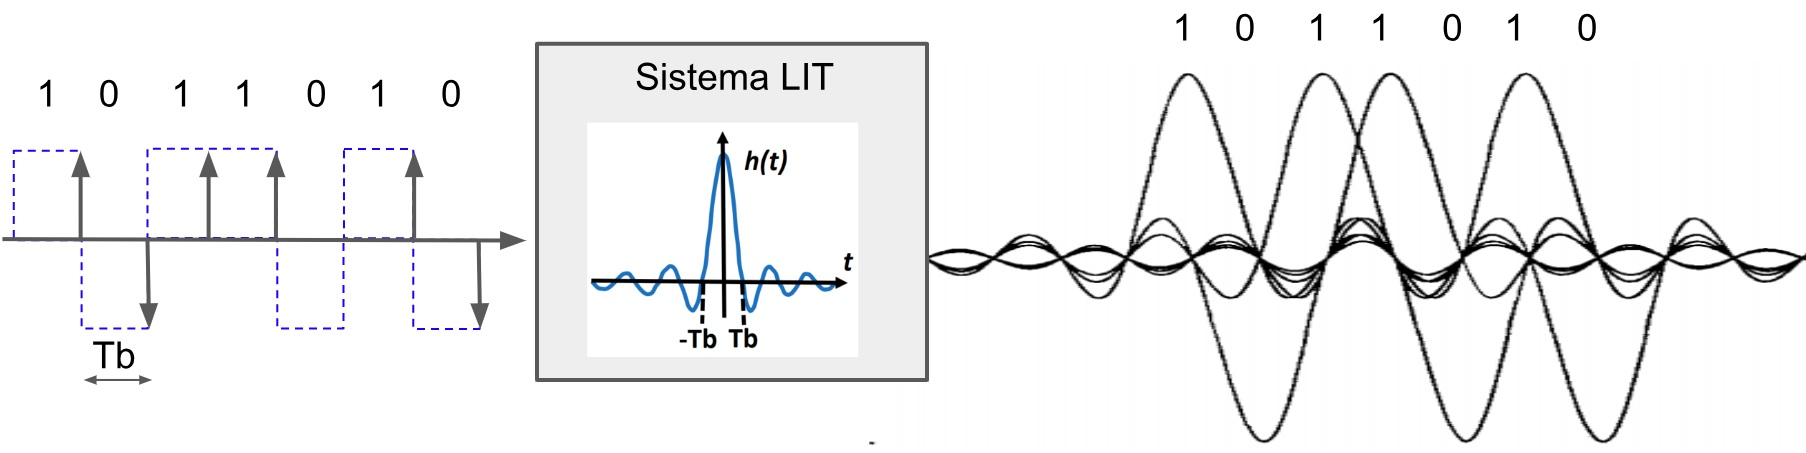
\includegraphics[scale=0.3]{Imagenes/filtro_nyquist.jpg}
	\label{fig:Secuencia}
	%	\captionsetup{justification=raggedright,font={scriptsize,bf,it}}
	%	\caption*{fuente: Tomado de Haykin}
\end{figure}

Solo resta definir cual es la respuesta al impulso del sistema LIT. Ya se ha dicho que los pulsos tienen que tomar la forma de una función sinc(..). Como se aprecia en la Figura  \ref{fig:Secuencia}, los pasos por cero deben darse cada periodo de tiempo $T_b$ de modo que la respuesta al impulso es la siguiente:

\begin{equation} \label{capcuatro_trece}
	 h(t) = sinc(\dfrac{t}{T_{b}}) 
\end{equation}

\subsubsection{Implementación del Filtro de Nyquist en versión Discreta}
La idea es que cada bit es previamente representado como un delta discreto, con amplitud 1 para los unos y con amplitud -1 ó 0 para los ceros. Esto es lo más normal en cualquier sistema discreto implementado como un programa de software como en GNU Radio. En este caso, la respuesta al impulso toma una forma discreta $h[n]$. El único problema es que en la práctica, la respuesta al impulso no puede tener una duración infinita como es el caso de h(t) (ver la Figura \ref{fig:Eme}). Esto impacta a la respuesta en frecuencias que ya deja de ser tan idealmente rectangular.  \\

Implicaciones en el ancho de banda :

\vspace{200px}
\begin{figure}[h!]
	\captionsetup{justification = raggedright, singlelinecheck = false}
	\caption{Respuesta al impulso de un Filtro de Nyquist. En color rojo el caso de un Filtro de Nyquist discreto} 
	\centering
	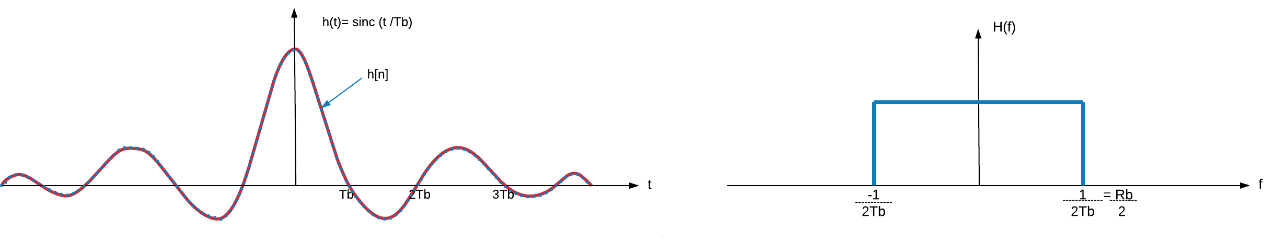
\includegraphics[scale=0.5]{Imagenes/Eme.png}
	\label{fig:Eme}
	%	\captionsetup{justification=raggedright,font={scriptsize,bf,it}}
	%	\caption*{fuente: Tomado de Haykin}
\end{figure}

En adelante $W=\frac{R_b}{2}$ es el ancho de banda según el criterio de Nyquist:

\begin{equation} \label{capcuatro_catorce}
	 h(t) = sinc(2Wt) = \dfrac{sin(2\pi Wt)}{2\pi Wt}
\end{equation}

El paso a la versión discreta puede hacerse teniendo en cuenta que $t=nT_s$ , donde Tses el periodo de muestreo, $T_s = \frac{T_b}{Sps} $, donde $Sps$ (Samples per symbol) es el número de muestras que caen en la duración del bit. \\

\begin{equation} \label{capcuatro_quince}
	 t = nT_s = \dfrac{nT_b}{Sps} = \frac{n}{R_{b}Sps} = \frac{n}{2WSps} 
\end{equation}

De modo que \\

\begin{equation} \label{capcuatro_diesiseis}
	 h[n] = sinc(\dfrac{2Wn}{2WSps}) = sinc(\frac{n}{Sps}) 
\end{equation}

Con lo cual se concluye que: El mínimo ancho de banda que requiere una señal binaria banda base es $W=\frac{R_b}{2}$, lo cual es lo mismo que decir que la rata máxima de bits que puede enviar representados en una señal binaria por un canal banda base con Ancho de Banda W es Rb=2W. Es esta expresión en que el criterio de Nyquist se parece al Teorema de Nyquist, pero son cosas diferentes. \\

\subsection{El Criterio de Nyquist en las señales M-arias.}
Aplica de manera similar a las señales binarias. La diferencia está en que las señales binarias llevan bits y por lo tanto la duración de los bits es lo que cuenta. En las señales M-arias, se tienen símbolos y la duración de los símbolos es lo que cuenta. Por eso, en las señales M-arias se usa $R_s$, que es la rata de símbolos, es lugar de $R_b$.\\ 

\textcolor{red}{[Falta un ejemplo para mayor claridad. No solo sobre aplicación del Criterio de Nyquist, sino lo que significan las señales M-arias]}

\subsection{El Filtro Coseno Alzado}
El Filtro de Nyquist presenta algunos problemas: se trata de un filtro ideal y por lo tanto su implementación en la práctica sería apenas una aproximación. Sin embargo, este criterio ha establecido una meta que permite a los científicos buscar soluciones que se acerquen a este criterio. El codificador Duobinario es un filtro que logra ese objetivo, sin embargo, es más común el uso del filtro Coseno elevado, que no logra el mismo resultado, pero tiene mayor acogida por su sencillez. \\

Es posible superar las dificultades prácticas que se encontraron con el filtro de Nyquist o canal de Nyquist ideal extendiendo el ancho de banda desde W hasta un valor ajustable entre W y 2W. recordemos que $W = \frac{Rb}{2}$ corresponde al criterio de Nyquist. \\
Así, el Filtro Coseno Elevado tiene la respuesta al impulso

\begin{equation} \label{capcuatro_diesisiete}
	 h(t) = sinc(2Wt)\dfrac{cos(\alpha2\pi Wt)}{1-16\alpha ^{2}W^{2}t^{2}}
\end{equation}

En esta expresión, el denominador puede dar cero, cuando $1-16 \alpha^{2}W^{2}t^2=1$, es decir, cuando $\alpha = \frac{1}{4Wt}$. Por ello se usa también la expresión \\

\begin{equation} \label{capcuatro_diesiocho}
h(t)=\left \{ \begin{matrix}
\frac{\pi}{4}  sinc(\frac{1}{2 \alpha}) &, & t=\pm \frac{1}{4 \alpha W}=\frac{T_b}{2 \alpha} \\
\\ 
sinc(2Wt) \frac{cos(\alpha \pi 2Wt)}{1-16 \alpha^2 W^2 t^2} & , & otros \space casos 
\end{matrix} \right.
\end{equation}


Pasándola al dominio discreto, como se hizo para el criterio de Nyquist se obtiene \\

\begin{equation} \label{capcuatro_diesinueve}
h[n]=\left \{ \begin{matrix}
\frac{\pi}{4} sinc(\frac{1}{2 \alpha}) &, & n=\pm \frac{Sps}{2 \alpha} \\
\\ 
sinc(n/Sps) \frac{cos(\alpha \pi n/Sps)}{1-(2 \alpha n/Sps)^2} & , & otros \space casos 
\end{matrix} \right.
\end{equation}

\begin{figure}[h!]
	\captionsetup{justification = raggedright, singlelinecheck = false}
	\caption{Respuesta al impulso del Filtro Coseno Alzado para diferentes valores de $\alpha$} 
	\centering
	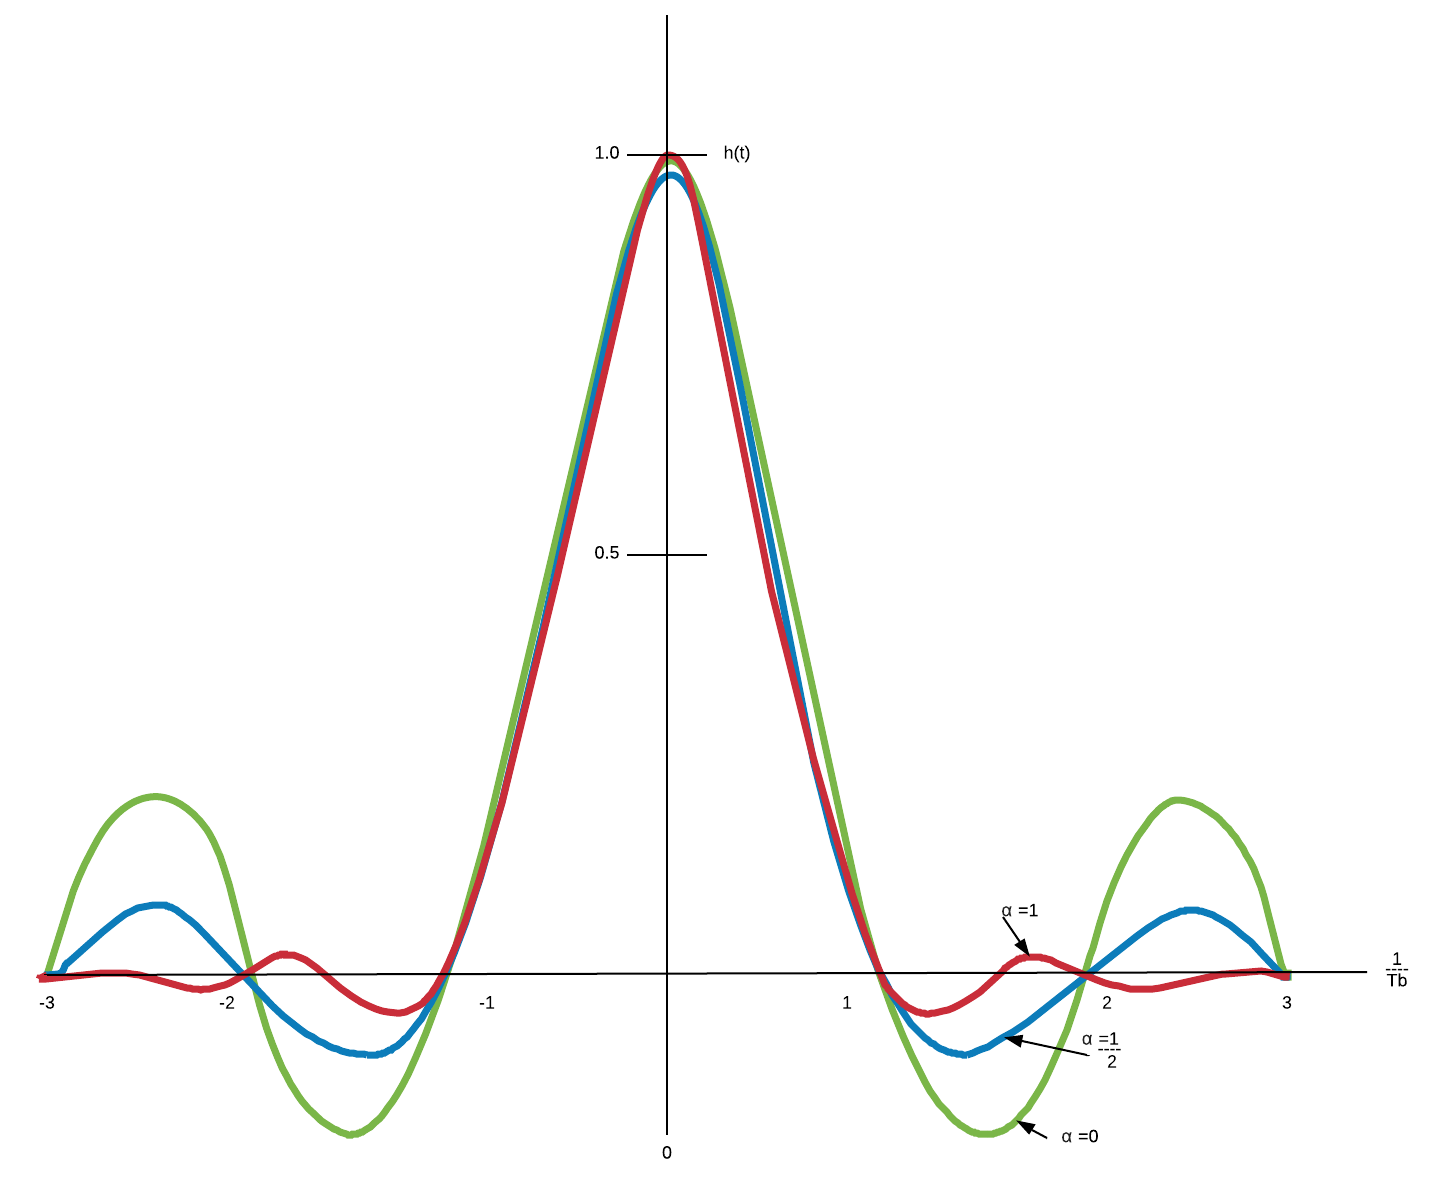
\includegraphics[scale=0.3]{Imagenes/Seno.png}
	\label{fig:Seno}
	%	\captionsetup{justification=raggedright,font={scriptsize,bf,it}}
	%	\caption*{fuente: Tomado de Haykin}
\end{figure}

$ \alpha $ es conocido como el rolloff factor, que en español significa factor caída. En GNU radio se usa el término en inglés. La respuesta en frecuencias del filtro Coseno Alzado está dada por la siguiente expresión: \\

\begin{equation} \label{capcuatro_veinte}
H(f)=\left \{ \begin{matrix}
1 &, & |f|  \leq W(1- \alpha) \\
\\ 
\dfrac{1}{2} [1+cos(\frac{\pi}{2W \alpha}[|f|-W(1-\alpha)])] & , & W (1- \alpha)  <  |f| \leq W(1+\alpha) \\
 \\
0 & , & resto
 
\end{matrix} \right.
\end{equation}

El caso más común es cuando $\alpha = 1 $ y se dice que se tiene el coseno elevado con toda su caída (full rolloff)”. Con el full rolloff la la respuesta en frecuencia es: \\

\begin{equation} \label{capcuatro_veintiuno}
	 H(W) = \dfrac{1}{4W}[1+Cos(\frac{\pi f}{2W})] \space , 0 < |f| < 2W,\space  0 para otros valores de f
\end{equation}

En todo caso, la respuesta en frecuencia para otros valores se puede tomar de la Figura \ref{fig:Coseno-elevado}. \\

%\vspace{200px}
\begin{figure}[h!]
	\captionsetup{justification = raggedright, singlelinecheck = false}
	\caption{Respuesta en frecuencia del Filtro Coseno Alzado para varios valores de $\alpha $} 
	\centering
	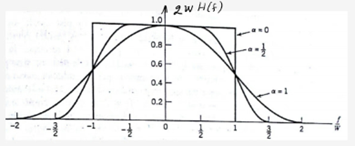
\includegraphics[scale=1.2]{Imagenes/Coseno-elevado.png}
	\label{fig:Coseno-elevado}
	%	\captionsetup{justification=raggedright,font={scriptsize,bf,it}}
	%	\caption*{fuente: Tomado de Haykin}
\end{figure}

Con el filtro Coseno Elevado se requiere entonces un ancho de banda igual a Rb para $\alpha =1$ . Con GNU Radio usualmente se emplea este filtro con un rolloff de $\alpha=0,5$ o de $\alpha =1$. Ver más detalles en el libro de Haykin [17], capítulo 4.5, \textcolor{Red}{página 261.}\\
Para mostrar una escala de frecuencia no normalizada como se ha hecho con las anteriores gráficas, a continuación se comparte una imagen tomada de wikipedia, donde el factor de caída está representado como $ \beta $ : \\

En GNU Radio se usa tanto el término Roll Off Factor como Excess Bandwidth para hacer referencia al mismo coeficiente. El término Excess Bandwidth se refiere al número de veces que el ancho de banda elegido supera al ancho de banda de Nyquist W. \\

\vspace{300px}
\begin{figure}[h!]
	\captionsetup{justification = raggedright, singlelinecheck = false}
	\caption{Respuesta en Frecuencia del Filtro (arriba) y Respuesta al Impulso (abajo)} 
	\centering
	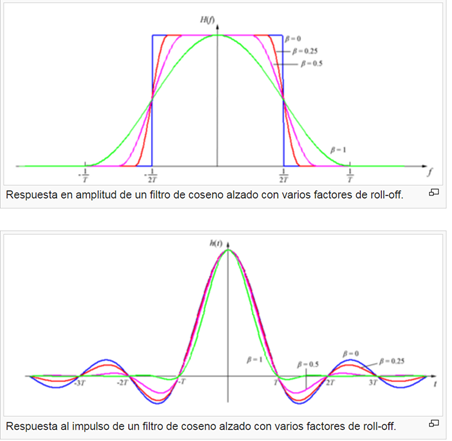
\includegraphics[scale=0.8]{Imagenes/Roll-off.png}
	\label{fig:Roll-off}
	%	\captionsetup{justification=raggedright,font={scriptsize,bf,it}}
	%	\caption*{fuente: Tomado de Haykin}
\end{figure}

\subsection{Implementación en GNU Radio del Filtro Formador de Pulsos}

En GNU Radio el Wave Forming es también un paso necesario cuando se tiene una señal digital. La diferencia es que esa señal será compleja ya que se tratará de una señal que espera el Up Converter, el cual a su vez se encuentra en el Hardware de una solución SDR. Antes de llegar al Up converter la señal debe pasar por un conversor digital análogo (DAC) como es el caso del hardware usado en el NI USRP 2920 visto en el capítulo  1 y que se resume en la figura siguiente.\\

%\vspace{200px}
\begin{figure}[h!]
	\captionsetup{justification = raggedright, singlelinecheck = false}
	\caption{ El Wave Forming como intermediario entre el Modulador y el DAC.} 
	\centering
	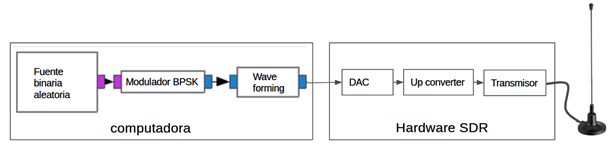
\includegraphics[scale=1]{Imagenes/Wave.png}
	\label{fig:Wave}
	%	\captionsetup{justification=raggedright,font={scriptsize,bf,it}}
	%	\caption*{fuente: llllll}
\end{figure}

En la figura \ref{fig:BPSK} se tiene un ejemplo de la señal que entrega un modulador digital BPSK en gnuradio, la cual es compleja por tratarse de la versión bandabase. Como puede verse, esa señal está un tanto alejada de la correspondiente en el mundo real, que son los cuadros que aparecen punteados en la figura  \ref{fig:BPSK}. 

\vspace{200px}
\begin{figure}[h!]
	\captionsetup{justification = raggedright, singlelinecheck = false}
	\caption{Ejemplo de la señal que entrega el modulador BPSK.} 
	\centering
	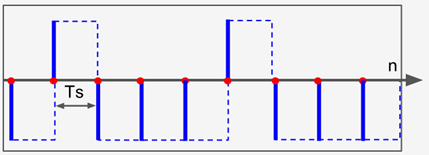
\includegraphics[scale=1]{Imagenes/BPSK.png}
	\label{fig:BPSK}
		\captionsetup{justification=raggedright,font={scriptsize,bf,it}}
		\caption*{Nota: En línea azul grueso la componente real, en rojo la imaginaria, en punteada la que corresponde en el mundo físico. Ts - duración del símbolo}
\end{figure}
\subsubsection{Wave Forming basado en pulsos rectangulares}
En la Figura \ref{fig:Azul}, en color azúl muestra la señal que se podría tener a la salida del bloque Wave Forming si este se configura para que cada símbolo se repita cuatro veces en la misma duración Ts. Entonces, se obtiene una señal con una frecuencia de muestreo 4 veces mayor a la anterior la cual es más parecida a la esperada en el mundo real. \\

%\vspace{100px}
\begin{figure}[h!]
	\captionsetup{justification = raggedright, singlelinecheck = false}
	\caption{En línea azul la componente real y en rojo la señal a la salida del bloque Wave Forming. En negro la salida del DAC. Sps=4} 
	\centering
	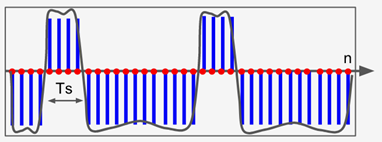
\includegraphics[scale=1]{Imagenes/Azul.png}
	\label{fig:Azul}
%	\captionsetup{justification=raggedright,font={scriptsize,bf,it}}
%	\caption*{Nota: En línea azul grueso la componente real, en rojo la imaginaria, en punteada la que corresponde en el mundo físico. Ts - duración del símbolo}
\end{figure}

El DAC entrega como resultado la señal que aparece en color negro para la parte real y una de nivel cero para la parte imaginaria. Tampoco se ha logrado reproducir la señal continua en forma ideal como la mostrada en forma punteada en la Fig.1, ya que esa señal tendría un espectro de ancho de banda infinito, lo que significa que es necesario que haya infinitas muestras por bit en la señal que se entrega al DAC, lo cual es imposible desde todo punto de vista. Se obtiene más bien una señal que tiene una forma similar a la esperada y que de paso tiene un ancho de banda finito igual a:

\begin{equation} \label{capcuatro_veintidos}
	 BW = \frac{samp-rate}{2}=\frac{Sps}{2T_{s}} 
\end{equation}

Donde samp-rate es la frecuencia de muestreo de la señal que entra al ADC y Sps es el número de muestras por símbolo, del inglés samples per symbol, lo cual es coherente con el Teorema de Nyquist.
\textcolor{red}{falta un ejemplo con gnuradio que muestre cómo son las cosas no solo en tiempo, sino en frecuencia, diagrama de ojo, etc. Incluso sería util ofrecer el codigo de python para producir este filtro}
\subsubsection{Wave Forming basado en el criterio de Nyquist}
\textcolor{red}{Falta este tema}

\subsubsection{Wave Forming basado en el criterio Coseno Alzado}
\textcolor{red}{Falta este tema}

\subsection{Regeneracion de Bits}
La regeneración de los bits es el procedimiento para recuperar en el receptor los bits transmitidos, luego de haber pasado por un canal. En el caso más sencillo se trata simplemente de realizar un muestreo a cada bit para obtener un nivel de señal que luego pasa a un bloque un comparador donde se tiene una referencia o umbral de comparación para producir un uno o un cero según corresponda con la comparación.\\

%%%%%%%%%%%%%%%%%%%%%%%%%%%%%%%%%%%%%%%%%%%%%%%%%%

\section{Consecuencias del desvanecimiento}

La dificultad que surge con la permanente presencia de ruido en un canal de comunicaciones. De modo que cuando la señal emitida se va desvaneciendo en su trayectoria, disminuye la relación señal a ruido que se percibe en el receptor. En la Figura \ref{fig:Ruido-canal} se muestra este efecto para el caso de una señal BPSK vista en banda base. Es decir, la señal puede viajar en pasobandas, pero es observada por un USRP en forma de envolvente compleja, aunque en la se ha mostrado solo la componente real ya que en BPSK la imaginaria es cero. Esta señal es también común en comunicaciones por cable de cobre sin usar modulación pasobandas, mostrando en este caso solo la componente real.

\begin{figure}[h!]
	\captionsetup{justification = raggedright, singlelinecheck = false}
	\caption{Afectacion de la relación Señal a Ruido por el efecto de desvanecimiento} 
	\centering
	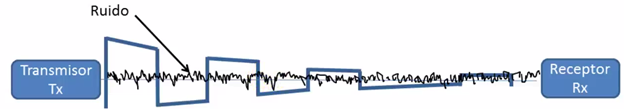
\includegraphics[scale=1]{Imagenes/Ruido-canal.png}
	\label{fig:Ruido-canal}
	%	\captionsetup{justification=raggedright,font={scriptsize,bf,it}}
	%	\caption*{fuente: \textcolor{
	%			Orange}{Tomada de Wikipedia}}
\end{figure}


%%%%%%%%%%%%%%%%%%%%%%%%%%%%%%%%%%%%%%%%%%%%%%%%%%%%%

\section{Consecuencias del Fenómeno de Multitrayectoria}



\subsection{El Jitter}
La distorsión producida por el fenómeno de multitrayectoria puede ser intra-símbolo, cuando el efecto de las reflexiones es más corto que la duración de los símbolos, pero también se da el caso de que sea intersimbolo (ISI) debido al retardo que pueden tener ciertas reflexiones y a la deformación que ocurre en el dominio de las frecuencias, entonces los bits o los símbolos puede resultar superpuestos en el receptor, lo que también se conoce como Jitter. \\

El término Jitter es un poco más amplio, pues no es exclusivo para el fenómeno de multitrayectoria. Se denomina jitter (término inglés para fluctuación) a la variabilidad temporal durante el envío de señales digitales, una ligera desviación de la exactitud de la señal de reloj puede producirlo. El jitter puede ser una de las consecuencias del fenómeno de multi trayectoria que siguen las ondas en su propagación desde el transmisor al receptor. En la la televisión digital terrestre (TDT), con el standard DVB-T2, el Jitter es algo muy propio del sistema, pues este sistema ha sido pensado para lograr que cada operador use frecuencias únicas en todo el territorio asignado (SFN, de single frequency network). En este caso, el operador despliega las estaciones de radiodifusión que sean necesarias para cubrir todo el territorio asignado. Entonces, como todas las estaciones deben radiar la misma señal, a un punto de interés llega no solo la señal de la antena más cercana sino aportes de otras antenas, con lo cual la señal se ve afectada por el Jitter que depende de la geografía y la distancia en que se encuentre el receptor. El Jitter es algo no deseado, es inevitable, pero puede ser premeditado como en el caso de la TDT. \\

\begin{figure}[h!]
	\captionsetup{justification = raggedright, singlelinecheck = false}
	\caption{Red de Frecuencias Únicas en TDT} 
	\centering
	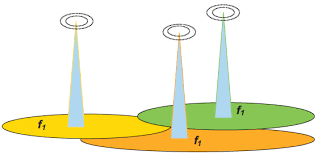
\includegraphics[scale=1]{Imagenes/Jitter.png}
	\label{fig:Jitter}
	%	\captionsetup{justification=raggedright,font={scriptsize,bf,it}}
	%	\caption*{Fuente: tomado de F. Pérez Fontán} 
\end{figure}

En ese caso, cómo se tienen varias áreas o celdas cubiertas con la misma banda de frecuencias, radiando la misma señal, pueden llegar a interferirse en ciertas zonas, lo importante es que el Jitter no sobrepase unos valores que hagan que la señal útil sea irrecuperable. El jitter puede estar variando, como se muestra en la siguiente figura donde Aj refleja esa variabilidad que se da cuando varía el canal, por ejemplo, porque el usuario o las fuentes reflectoras se mueven \\

%\vspace{200px}
\begin{figure}[h!]
	\captionsetup{justification = raggedright, singlelinecheck = false}
	\caption{El Jitter} 
	\centering
	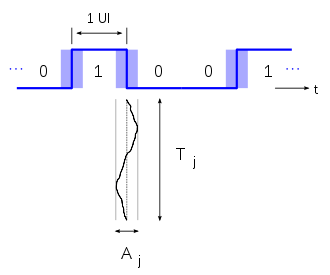
\includegraphics[scale=1]{Imagenes/Intersimbolo.png}
	\label{fig:Intersimbolo}
	%	\captionsetup{justification=raggedright,font={scriptsize,bf,it}}
	%	\caption*{Fuente: tomado de F. Pérez Fontán} 
\end{figure}

También es claro que el Jitter es una de las causas de lo que se conoce como Interferencia Intersimbolo (ISI) pues finalmente lo que se observa es que la energía de unos símbolos se solapa con la de otros, pero en muchos casos al Jitter se le puede dar un tratamiento especial, diferente a la ISI producida por las restricciones de ancho de banda del canal, cuando el Jitter puede ser visto como una inestabilidad en la frecuencia en que llegan los símbolos al receptor, lo cual se traduce en la necesidad de realizar un timing o clock recovery, pero de manera continuada o adaptativa. \\



\subsection{Desvanecimientos lentos y rápidos. Efecto de Rayleigh}
Consecuencias del desvanecimiento rápido: \\
En un sistema de comunicaciones digitales basado en GNU Radio, este fenómeno se verá como una tembladera de las constelaciones rápida, pero con pocas desviaciones. En la siguiente figura hay un ejemplo visto en dos instantes de tiempo, donde se observa que la nube de puntos de una constelación se ha movido ligeramente de su posición. En una observación continua veremos entonces las constelaciones danzando en alrededor de la posición original. \\


\begin{figure}[h!]
	\captionsetup{justification = raggedright, singlelinecheck = false}
	\caption{Consecuencias en la constelación del Desvanecimiento rápido} 
	\centering
	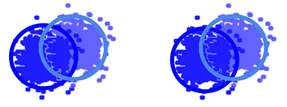
\includegraphics[scale=1]{Imagenes/Circulos.png}
	\label{fig:Circulos}
	%\captionsetup{justification=raggedright,font={scriptsize,bf,it}}
%	\caption*{fuente: Tomado de F. Pérez Fontán\textbf{Nota:}Esta no es la señal recibida sino lo que entrega un medidor de nivel de potencia} 
\end{figure}

Consecuencias del desvanecimiento lento. En la Figura \ref{fig:Variacion} se presenta un ejemplo de lo que puede ocurrirle a a una constelación BPSK.\\

\begin{figure}[h!]
	\captionsetup{justification = raggedright, singlelinecheck = false}
	\caption{Consecuencias en la constelación del Desvanecimiento lento} 
	\centering
	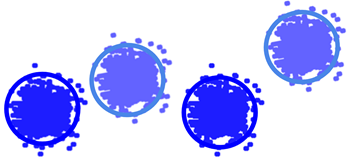
\includegraphics[scale=1]{Imagenes/Variacion.png}
	\label{fig:Variacion}
%	\captionsetup{justification=raggedright,font={scriptsize,bf,it}}
%	\caption*{Fuente: tomado de F. Pérez Fontán} 
\end{figure}



\subsection{Afectación por no linealidades}

Pero la multi trayectoria también trae consecuencias que son comunes en el paso de una señal por un medio no lineal, lo cual se ve principalmente reflejado en el dominio de las frecuencias, donde algunas frecuencias o rangos de frecuencia de la señal resultan más o menos amplificadas que otras.\\

\begin{figure}[h!]
	\captionsetup{justification = raggedright, singlelinecheck = false}
	\caption{Variaciones espectrales debido a no linealidades del canal} 
	\centering
	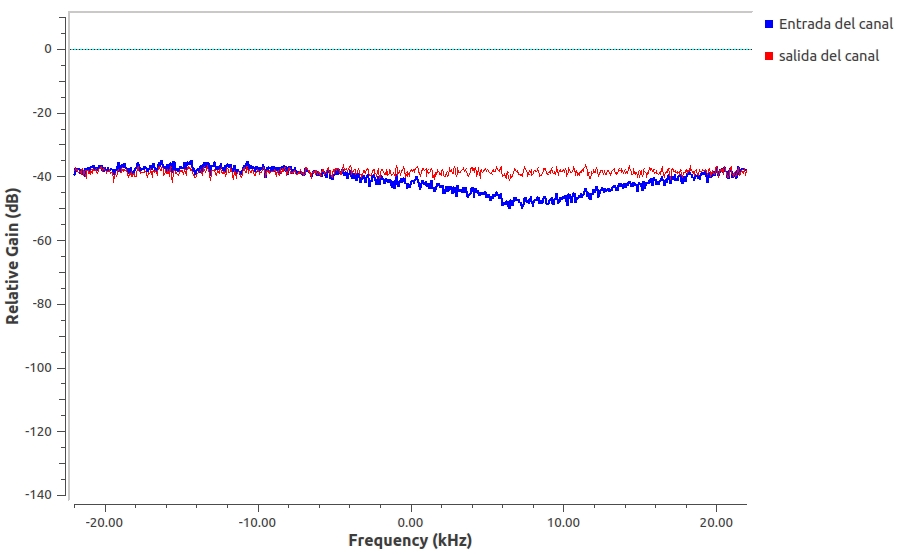
\includegraphics[scale=0.35]{Imagenes/canal_no_lineal.jpg}
	\label{fig:canal_no_lineal}
	%	\captionsetup{justification=raggedright,font={scriptsize,bf,it}}
	%\caption*{Fuente: tomado de:  \url{https://wiki.gnuradio.org}} 
\end{figure}
\begin{figure}[h!]
	\captionsetup{justification = raggedright, singlelinecheck = false}
	\caption{QPSK impactada por no linealidades del canal} 
	\centering
	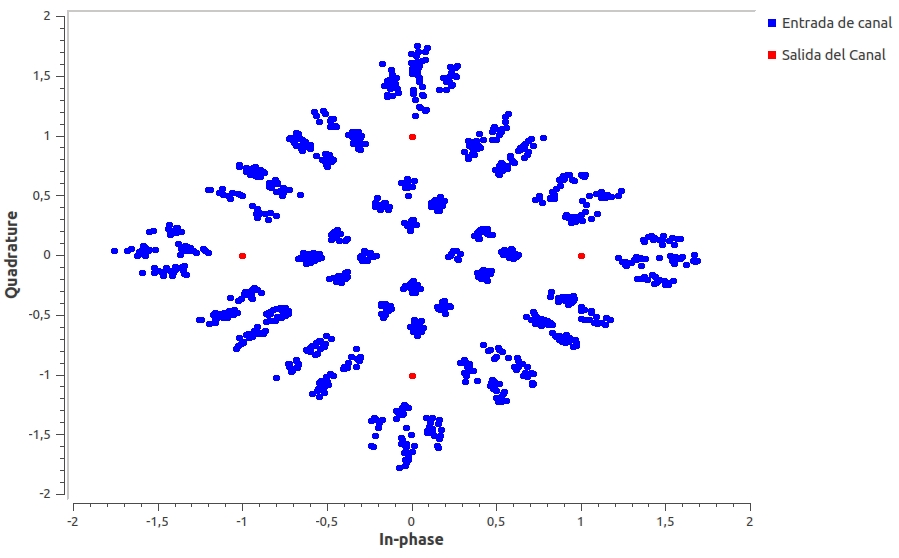
\includegraphics[scale=0.35]{Imagenes/qpsk_canal_no_lineal.jpg}
	\label{fig:qps_canal_no_lineal}
	%	\captionsetup{justification=raggedright,font={scriptsize,bf,it}}
	%\caption*{Fuente: tomado de:  \url{https://wiki.gnuradio.org}} 
\end{figure}

Para mostrar un ejemplo de esta afectación vamos al caso de SDR, con lo cual nos referiremos directamente a lo que ocurre con la Envolvente compleja. El ejemplo se presenta en la Figura \ref{fig:canal_no_lineal}, donde vemos que la señal que se origina en la parte transmisora tiene una PSD que es plana en todas las frecuencias. Para lograrlo, hemos conectado el medidor de PSD a la salida del modulador, antes del Formador de Pulsos, de modo que solo se tiene una muestra por símbolo, con lo cual la señal modulada pueda ser vista, desde el punto de vista espectral, como un ruido blanco. Otro medidor de la PSD lo hemos conectado en el receptor, pero no inmediatamente a la salida del canal sino después del proceso de muestreo que permite obtener solo una muestra por símbolo. Vemos que la señal recibida, en color rojo, tiene fuertes desviaciones de magnitud en el dominio de las frecuencias.\\
En la Figura \ref{fig:qpscanal_no_lineal} se presenta un ejemplo del impacto que las no linealidades del canal pueden tener sobre la forma la constelación de una señal con modulación QPSK y como podemos ver, resulta en una desfiguración que hace casi imposible reconocer directamente los símbolos.\\

Pero lo peor de esta afectación, es que no es estática sino que varía con el tiempo, lo cual se puede apreciar mediante un analizador de espectros configurado en modo waterfall para mostrar como el espectro varía en el tiempo, como se muestra en la Figura \ref{fig:waterfall_canal_no_lineal}
\begin{figure}[h!]
	\captionsetup{justification = raggedright, singlelinecheck = false}
	\caption{Waterfall para una señal QPSK afectada por no linealidades que varian en el tiempo} 
	\centering
	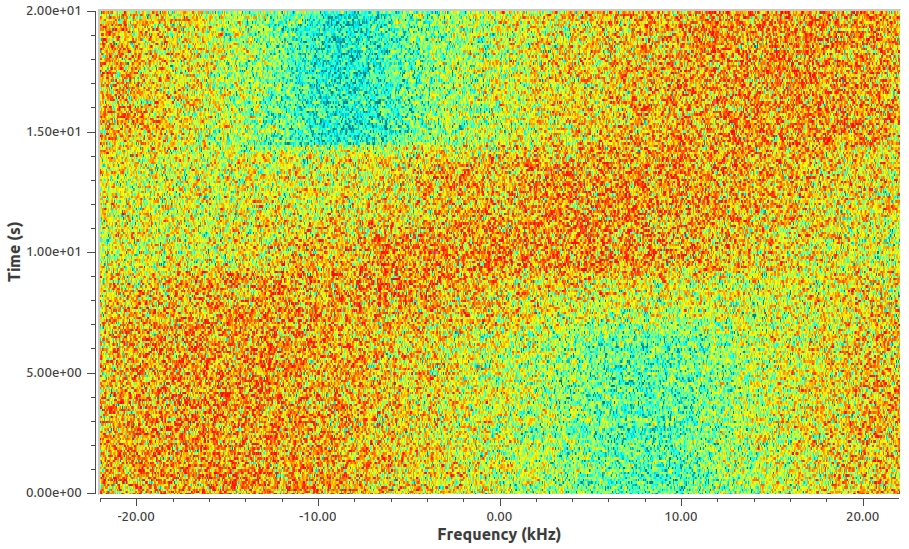
\includegraphics[scale=0.35]{Imagenes/waterfall_canal_no_lineal.jpg}
	\label{fig:waterfall_canal_no_lineal}
	%	\captionsetup{justification=raggedright,font={scriptsize,bf,it}}
	%\caption*{Fuente: tomado de:  \url{https://wiki.gnuradio.org}} 
\end{figure}
%%%%%%%%%%%%%%%%%%%%%%%%%%%%%%%%%%
\section{Consecuencias de otros Fenómenos}
\subsection{Desviación angular}
En términos de señal paso bandas, ser refiere a la desviación angular que existe entre dos señales. En la Figura \ref{fig:bpsk_desfasadas} se tiene un ejemplo para la modulación BPSK, donde la versión original está en color azul y la versión desfasada en 45 grados está en color rojo.\\

\begin{figure}[h!]
	\captionsetup{justification = raggedright, singlelinecheck = false}
	\caption{Señal BPSK y su versión desfasada en 45 grados} 
	\centering
	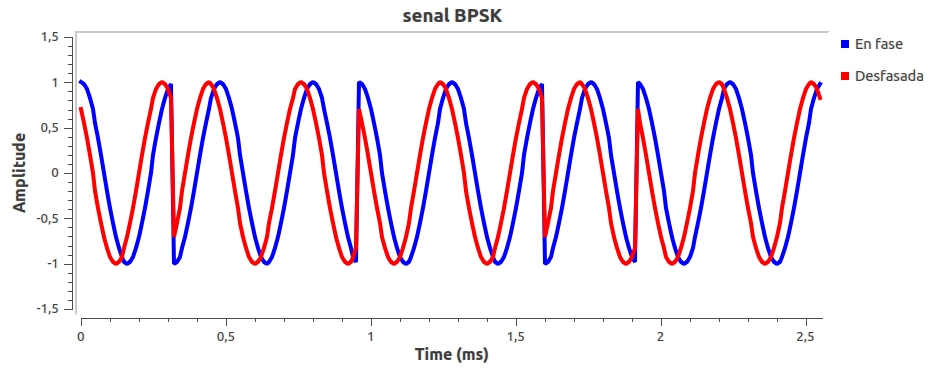
\includegraphics[scale=0.45]{Imagenes/bpsk_desfasadas.jpg}
	\label{fig:bpsk_desfasadas}
% Lo siguiene es para indicar la fuente de la cual fue tomada la figura
%  \captionsetup{justification=raggedright,font={scriptsize,bf,it}}
%  \caption*{fuente: Tomada de Wikipedia}
\end{figure}
En la Figura \ref{fig:bpsk_desfasadas90} se tiene otro ejemplo para el caso en que el desfase es de 90 grados. En los sistemas de comunicación, el desfase es prácticamente un fenómeno obligatorio dado principalmente por el paso de la señal através de diferentes condiciones del medio de transmisión, que para nuestro caso es el canal inalámbrico. También se puede producir en el paso de la señal por diferentes circuitos de radio que se tienen tanto en los equipos de transmisión como de recepción. Incluso, aún en el caso hipotético en que la señal llegue sin desfase alguno, este puede aparecer al intentar bajar la señal a bandabase, ya que es poco probable que la fase del oscilador local del down converter esté en fase con la señal recibida.  
\begin{figure}[h!]
	\captionsetup{justification = raggedright, singlelinecheck = false}
	\caption{Señal BPSK y su versión desfasada en 90 grados} 
	\centering
	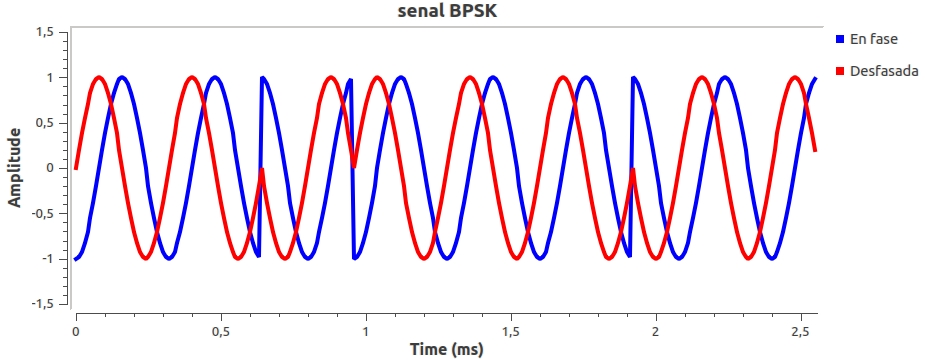
\includegraphics[scale=0.45]{Imagenes/bpsk_desfasadas90.jpg}
	\label{fig:bpsk_desfasadas90}
% Lo siguiene es para indicar la fuente de la cual fue tomada la figura
%  \captionsetup{justification=raggedright,font={scriptsize,bf,it}}
%  \caption*{fuente: Tomada de Wikipedia}
\end{figure}

Cuando se usan las técnicas de SDR la desviación de fase que llega al receptor no alcanza a ser corregida completamente en el hardware, de manera que se presenta en la Envolvente Compleja discreta que se recibe. En la Figura \ref{fig:16qam_desfasadas} se presenta un ejemplo para el caso de la modulación 16QAM, en la parte superior se tiene la constelación generada en el modulador de la parte transmisora, en la parte inferior está la constelación que se obtiene en el receptor cuando se presenta la desviación angular.\\
\begin{figure}[h!]
	\captionsetup{justification = raggedright, singlelinecheck = false}
	\caption{Constelación de la Modulación 16QAM y su versión con desviación de fase} 
	\centering
	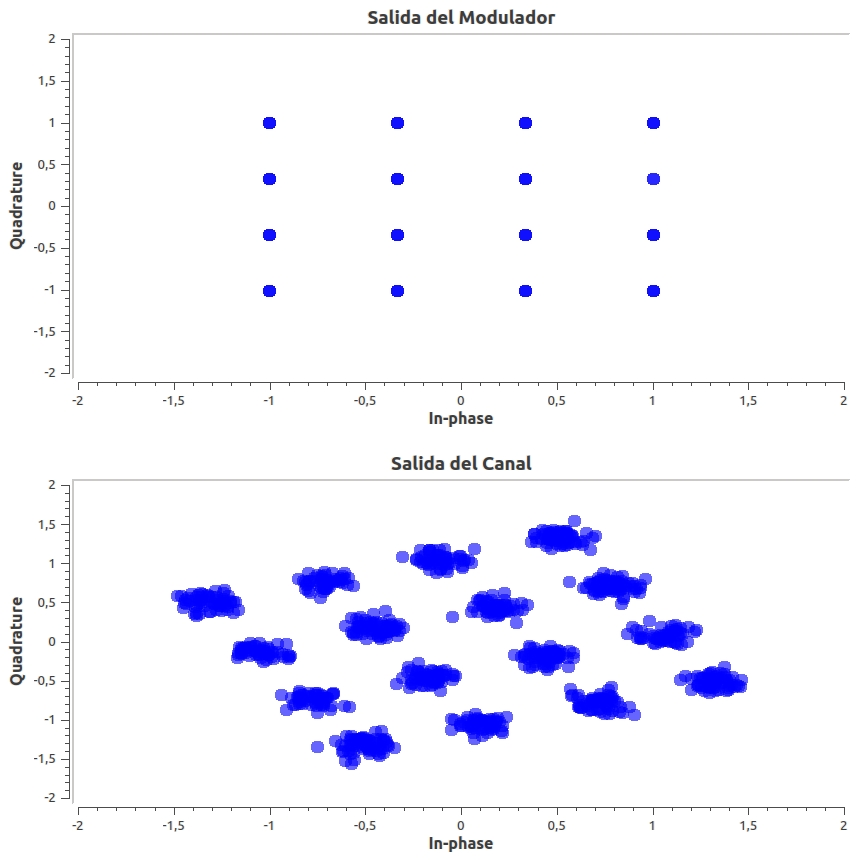
\includegraphics[scale=0.45]{Imagenes/16qam_desfasadas.jpg}
	\label{fig:16qam_desfasadas}
\end{figure}

La implementación de un simulador de un canal banda base con desviación de fase puede realizarse de la siguiente manera:
\begin{equation} \label{equ:p_dev}
	 z(t) = s(t)e^{j\phi}				
\end{equation}
donde $s(t)$ es la envolvente compleja de la señal que el transmisor entrega al canal; $\phi$ es el desfase que introduce el canal; y $z(t)$ es la salida del canal. 
\subsection{Desviación en frecuencia}
Las desviaciones entre la frecuencia usada en la transmisión y la que llega a un receptor, luego de que la señal atraviesa un canal, son también un fenómeno casi obligado, sobre todo cuando el canal es inalámbrico. La causa principal es el Efecto Doppler, aunque pueden haber otras como por ejemplo las imperfecciones en  los circuitos que generan la portadora tanto en el transmisor como en el receptor. En la Figura \ref{fig:bpsk_desv_frec} se presenta un ejemplo, donde la señal en color rojo aparece dos veces desviada de la original, sin embargo, en la práctica esta desviación suele ser de unos pocos Hertz.
\begin{figure}[h!]
	\captionsetup{justification = raggedright, singlelinecheck = false}
	\caption{Desvición Frecuencias entre dos señales BPSK} 
	\centering
	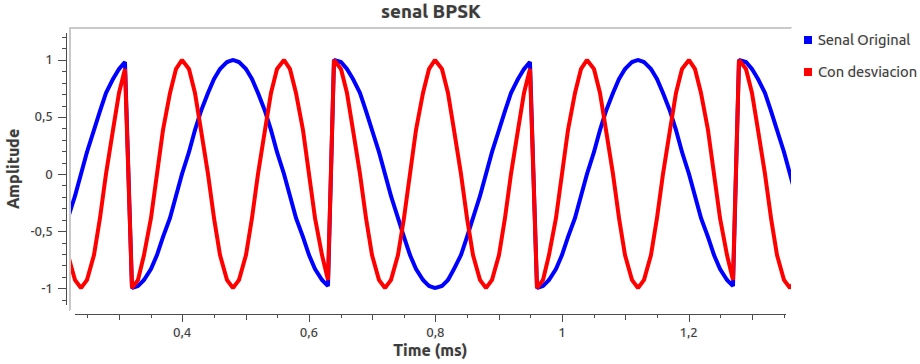
\includegraphics[scale=0.4]{Imagenes/bpsk_desv_frec.jpg}
	\label{fig:bpsk_desv_frec}
\end{figure}
Como en el caso de la desviación de fase, al usar técnicas de SDR, las desviaciones de frecuencias no alcanzan a ser corregidas completamente con el hardware, de modo que es un problema que se traslada a las componentes de software. En este sentido, nos ocuparemos ahora en conocer cómo es la envolvente compleja de una señal con desviación de frecuencias comparada con una sin ella. En este caso, la desviación está dada por la siguiente expresión: 
\begin{equation} \label{equ:f_dev}
	 z(t) = s(t)e^{j2\pi f_{desv} t}				
\end{equation}
donde $s(t)$ es la envolvente compleja de la señal que el transmisor entrega al canal; $f_{desv}$ es la desviación de frecuencia que introduce el canal; y $z(t)$ es la salida del canal.\\
Desde este punto de vista, es fácil deducir que una señal con desviación de frecuencias, puede ser observada a la salida del Down Converter como una constelación similar a la mostrada en la Figura \ref{fig:16qam_desfasadas} pero no estática, sino girando en contra de las manecillas del reloj si la desviación es positiva o en favor de las manecillas del reloj si es negativa. 
%%%%%%%%%%%%%%%%%%%%%%%%%%%%%%%%%%%%%%%%%%%%%%%%%%%%%

\section{Simulación de un canal inalámbrico en GNU Radio}

Simular el canal resulta tremendamente útil. Supongamos que vamos a implementar un método para corregir los estragos que produce la multitrayectoria. Para probar ese método es necesario contar con un canal en el cual se puedan aislar los fenómenos que no sean de multitrayectoria. Eso es posible cuando se cuenta con un canal simulado. Podemos ver el canal como un sistema que tiene una señal de entrada y una salida: la primera es la señal que entrega el equipo de transmisión y la segunda es la que entrega el equipo de recepción que obviamente estará afectada por los fenómenos de propagación. Como tanto el transmisor como el receptor operan con la envolvente compleja, resulta lógico que el canal sea implementado en banda base para lo cual es necesario poder llevar a banda base los efectos que pueden ocurrir a la señal paso bandas. En la figura siguiente se presenta el esquema de un canal realizado en GNU Radio.

%	\setcounter{figure}{106}
\vspace{200px}
\begin{figure}[h!]
	\captionsetup{justification = raggedright, singlelinecheck = false}
	\caption{Flujograma para el canal Inalámbrico} 
	\centering
	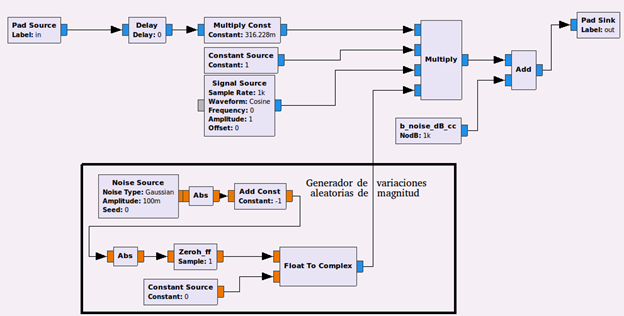
\includegraphics[scale=0.9]{Imagenes/Bloques.png}
	\label{fig:Bloques}
	%	\captionsetup{justification=raggedright,font={scriptsize,bf,it}}
	%	\caption*{fuente: \textcolor{
	%			Orange}{Tomada de Wikipedia}}
\end{figure}


\begin{itemize}
	\item [$\bullet$] \textbf{Bloques “Pad Source” y “Pad Sink”:} son los puertos de entrada y salida del canal
	\item [$\bullet$] \textbf{Bloque “Delay”:} permite configurar el retardo que puede estar produciendo el canal a la señal recibida. Si este valor cambia en el tiempo puede simular en cierta manera la presencia de Jitter.
	\item [$\bullet$]\textbf{Bloque “Multiply Const”:}permite configurar las pérdidas que el canal introduce, aunque este bloque no resulta muy necesario si lo que se requiere es lograr una cierta relación señal a ruido 
	\item [$\bullet$]\textbf{Bloque “Constant Source”:}  Permite configurar una desviación de fase que se presenta en cualquier caso en un canal, principalmente por componentes no lineales, por retardos o por falta de sincronismo entre el transmisor y el receptor. 
	\item [$\bullet$] \textbf{Bloque “Signal Source”:} Permite configurar una desviación de frecuencias, como la que puede presentarse por el Efecto Doppler o simplemente porque puede no coincidir exactamente la frecuencia usada en el transmisor con la usada en el receptor
	\item [$\bullet$] \textbf{Bloque “Multiply”:}  reúne todas las desviaciones multiplicativas que se aplican a la señal de recibida
	\item [$\bullet$]\textbf{Bloque “b-noise-dB-cc”:} agrega ruido blanco aditivo a la señal que entrega el canal. Gracias a esto se puede configurar la relación señal a ruido que se puede producir con la propagación de la onda
	\item [$\bullet$] En la parte inferior se tiene una interconexión para generar variaciones aleatorias de magnitud como las que se producen por el efecto de Rayleigh. 
	
\end{itemize}

\section{Técnicas para corregir los efectos del canal inalámbrico}
\subsection{El Filtro de Acoplamiento}
Los filtros de acoplamiento son totalmente necesarios en un receptor de señales digitales. A continuación, se describe el problema que conlleva a su uso. Este tema se analiza aquí para las señales binarias, pero fácilmente puede deducirse que aplica para símbolos de cualquier señal digital basada en constelaciones.  La figura 8 resume de la manera más sencilla posible como una señal digital binaria emitida g(t) desde un transmisor es afectada por ruido blanco aditivo, antes de pasar a un sistema de regeneración que se encuentra en el receptor. El sistema presentado en la figura sugiere la necesidad de usar un Filtro Lineal e Invariante en el Tiempo (LIT) para atenuar el efecto del ruido o para lograr elevar de alguna manera la relación señal a ruido antes de tomar una decisión sobre la presencia de un uno o un cero en un instante determinado. \\

%\setcounter{figure}{62}
\begin{figure}[h!]
	\captionsetup{justification = raggedright, singlelinecheck = false}
	\caption{Receptor Lineal} 
	\centering
	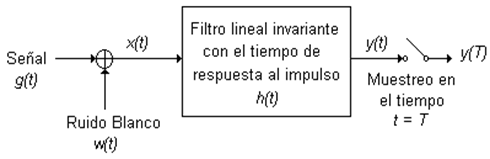
\includegraphics[scale=1]{Imagenes/Receptor.png}
	\label{fig:Receptor}
	%	\captionsetup{justification=raggedright,font={scriptsize,bf,it}}
	%	\caption*{fuente: Tomado de Haykin}
\end{figure}

Usualmente la señal recibida pasa por una etapa de acondicionamiento que permite resaltar un instante de tiempo, dentro de la duración de cada bit, en el cual la relación señal a ruido es máxima.\\

\begin{figure}[h!]
	\captionsetup{justification = raggedright, singlelinecheck = false}
	\caption{Filtro LIT usado como Filtro de Acoplamiento.\textcolor{blue}{El Formador de pulso es el mismo Filtro de Transmisión} } 
	\centering
	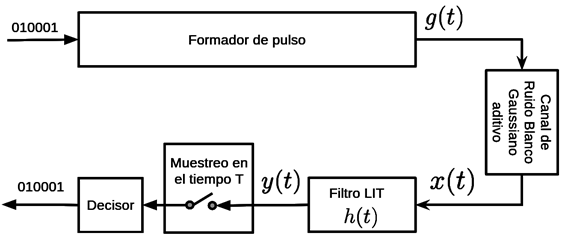
\includegraphics[scale=1]{Imagenes/Filtro.png}
	\label{fig:Filtro}
	%	\captionsetup{justification=raggedright,font={scriptsize,bf,it}}
	%	\caption*{fuente: Tomado de Haykin}
\end{figure}

La pregunta que surge es: \textbf{¿Para las condiciones dadas cómo debería ser ese filtro LIT? }\\ 

La respuesta $y(t)$ del filtro es la suma de la respuesta $g_0 (t)$ a la señal útil $g(t)$ y la respuesta $n(t)$ que resulta al pasar el ruido blanco w(t) a través de ese filtro, todo esto observado en la duración T de un un bit. Estamos suponiendo que a la entrada del Formador de Pulsos se tiene información en forma de bits, pero el análisis igual aplica para cuando allí se tienen símbolos que pueden incluso ser complejos, como los que entrega un modulador banda base: Entonces tenemos que: \\

\begin{equation} \label{capcuatro_veintitres}
	 y(t) = g_{0}(t) + n(t), 0  \leq t \leq  T  
\end{equation}

Sea $ \eta $ la relación entre el valor que toma $g_{0}(t)$en el instante óptimo T para el muestreo y la media cuadrática o potencia media del ruido.  se conoce mejor como Relación Señal a Ruido del Pulso Pico:

\begin{equation} \label{capcuatro_veinticuatro}
	 \eta = \dfrac{|g_{0}(T)|^{2}}{E[n^{2}(t)]} 
\end{equation}

En el libro de Haykin  \textcolor{Red}{[17]} se realiza un análisis para determinar la respuesta óptima $ h_{opt}(t) $ para el Filtro LIT que debe ser usado en el receptor para lograr el máximo valor   antes de pasar al proceso de regeneración de bits o símbolos. Lo que allí se logra demostrar es que para que  $ \eta = \eta_{max} $, la respuesta al impulso debe ser $ h_{opt}(t) = kg (T-t) $ o en el dominio de las frecuencias para $ \eta = \eta_{max} $,  $ h_{opt}(f) = kG(f)e^{-j2\pi fT} $ donde $ H_{opt}(t)$ es la transformada de Fourier de $ h_{opt}(t), G_{0}(f)$ es el conjugado de la transformada de Fourier de $g_{0}(t) $.

\begin{equation} \label{capcuatro_veinticinco}
	 y(t) = x(t)*h(t) = \int x(\tau)h(t-\tau)d\tau
\end{equation}

En la práctica se pueden usar los límites de integración entre $ -\infty y \infty$, pero también entre 0 y T si se desea reiniciar el proceso cada vez que ingresa un nuevo símbolo. En conclusión, la respuesta al impulso más óptima para el filtro, en las condiciones dadas, excepto por el valor de escala k, es la versión reflejada y atrasada de $g(t)$ que representa la forma del del pulso elegida para transmitir los símbolos de información que usualmente son bits. También puede decirse que en lugar de un Filtro LIT es posible usar un bloque que realiza la correlación que puede haber entre $x(t)$ y $g(t)$.

\begin{equation} \label{capcuatro_veintiseis}
	y(t) = x(t)oh(t) = \int x(t)h(t+\tau)d\tau
\end{equation}

Por esta razón se habla de acoplamiento entre la señal emitida y la usada en la recepción como respuesta al impulso para el Filtro LIT. También es claro que la autocorrelación es la misma convolución cuando h(t) tiene una forma simétrica \\

En una aplicación práctica podemos olvidarnos del desplazamiento T ya que solo tiene el efecto de producir un retardo en la respuesta, de modo también resulta válido decir que la operación de correlación entre la señal recibida y la forma de pulso g(t) usada en la transmisión es la manera forma más óptima para eliminar el ruido blanco. También podemos decir que si g(t) tiene una forma simétrica en el tiempo, se puede usar la operación de convolución en lugar de la correlación. \\

\subsubsection{Filtro de acoplamiento de pulsos rectangulares}

Aquí se analiza el caso ideal en que una señal pudiese ser emitida con una forma rectangular de Amplitud A y duración T. La siguiente figura muestra lo que ocurre cuando una señal rectangular $g(t)$ llega el receptor y luego pasa por el filtro de acoplamiento, se produce entonces la señal triangular $ g_0(t) $ que tiene un máximo en T  igual a $kA^{2}T$. También es posible deducir que es posible lograr un acoplamiento similar usando, en calidad de filtro, un integrador que se carga durante la señal y luego se descarga. En ambos casos el mejor instante para el muestreo es T. \\

\vspace{200px}
\begin{figure}[h!]
	\captionsetup{justification = raggedright, singlelinecheck = false}
	\caption{a) Pulso Rectangular; b) Salida del Filtro de Acoplamiento; c) Salida del Integrador } 
	\centering
	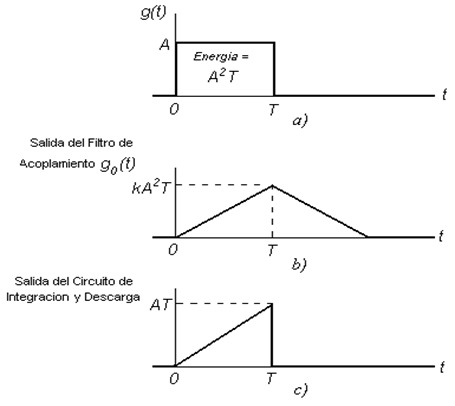
\includegraphics[scale=1]{Imagenes/Salida_filtro.png}
	\label{fig:Salida_filtro}
	%	\captionsetup{justification=raggedright,font={scriptsize,bf,it}}
	%	\caption*{fuente: Tomado de Haykin}
\end{figure}

El uso de un circuito de integración y descarga se muestra en el siguiente diagrama de bloques. \\

%\vspace{100px}
\begin{figure}[h!]
	\captionsetup{justification = raggedright, singlelinecheck = false}
	\caption{Filtro de acoplamiento basado en un circuito de Integración y Descarga } 
	\centering
	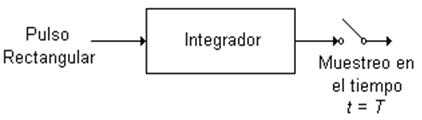
\includegraphics[scale=1]{Imagenes/Integrador.png}
	\label{fig:Integrador}
	%	\captionsetup{justification=raggedright,font={scriptsize,bf,it}}
	%	\caption*{fuente: Tomado de Haykin}
\end{figure}

En la siguiente figura se presenta el diagrama de ojo que ha sido obtenido en GNU Radio a la entrada y salida de un filtro de acoplamiento para señales digitales representadas como pulsos de forma cuadrada. \\

\vspace{200px}
\begin{figure}[h!]
	\captionsetup{justification = raggedright, singlelinecheck = false}
	\caption{Entrada (la gráfica superior) y salida (la inferior) de un Filtro de Acoplamiento para una señal con modulación BPSK usando GNU Radio } 
	\centering
	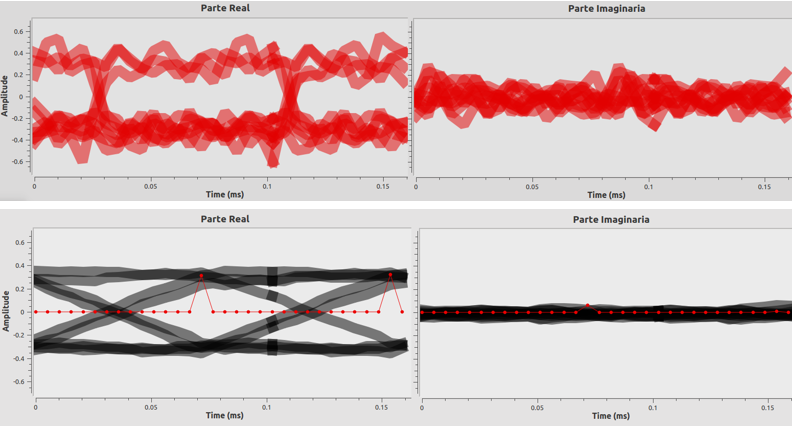
\includegraphics[scale=0.7]{Imagenes/Filtro-aco.png}
	\label{fig:Filtro-aco}
	%	\captionsetup{justification=raggedright,font={scriptsize,bf,it}}
	%	\caption*{fuente: Tomado de Haykin}
\end{figure}

\subsubsection{Filtro Raíz Cuadrada de Coseno Alzado}

Anteriormente se discutió el Filtro de Nyquist y el Filtro Coseno Alzado. El problema que surge ahora es: Si el transmisor usa un filtro de esos, ¿cuál sería el filtro de acoplamiento a usar en el receptor?\\ De acuerdo a la teoría vista sobre Filtro de acoplamiento, el filtro de acoplamiento a usar en el receptor debe tener, como respuesta al impulso, una forma reversada y atrasada de la forma de los pulsos usados en la transmisión. El problema que ahora surge es que, a la salida del filtro de acoplamiento, en el receptor, si bien se tiene un menor efecto del ruido blanco, ya no se van a obtener los instantes libres de ISI para cada símbolo, ya que al unir transmisor y receptor tenemos dos filtros Coseno Alzados en sería y por lo tanto la  Respuesta en Frecuencia resultante no será la misma que teníamos prevista para el Filtro Coseno Alzado. \\

La solución a este problema, consiste en usar en el transmisor un Filtro Raíz Cuadrada de Coseno Alzado (RRC de Root Raised Cosine), el cual tiene el siguiente efecto: La señal a la salida del Wave Forming, en el transmisor no tiene el instante libre de ISI, pero sí la PSD esperada, mientras en el receptor, a la salida del filtro de acoplamiento ya se tiene el instante libre de ISI, pues el Filtro RCC usado en el transmisor, seguido del Filtro RCC usado en el receptor, conformen de manera conjunta un Filtro RC. \\
Es importante tener en cuenta que la raíz cuadrada aplica a la respuesta en frecuencia, no en tiempo, de modo que:
Sí para el filtro Coseno Alzado se tiene:\\

\begin{equation} \label{capcuatro_veintisiete}
 	h_{RC}(t)\overset{TF}{\rightarrow}H_{RC}(f)
\end{equation}

Entonces, para el Filtro Raíz del Coseno Alzado se tiene la respuesta en frecuencia: \\

\begin{equation} \label{capcuatro_veintiocho}
	|H_{RRC}(f)|= \sqrt{|H_{RC}(f)|}
\end{equation}

Para cumplir esta condición en el dominio del tiempo, la respuesta al impulso del Filtro RRC resulta un tanto complicada: 

\begin{equation} \label{capcuatro_veintinueve}
	h(t)=\begin{cases}
	\frac{1}{T_{b}}(1+\alpha (\frac{4}{\pi}-1)) & \text{ ,   } t=0 \\ \\
	\frac{\alpha}{T_{b}\sqrt{2}}[(1+\frac{2}{\pi})sin(\frac{\pi}{4\alpha})+(1-\frac{2}{\pi})cos(\frac{\pi}{4\alpha})] & \text{ ,   } t= \pm\frac{T_{b}}{4\alpha}\\ \\
	\frac{1}{T_{b}}\frac{sin[\pi\frac{t}{T_b}(1-\alpha)]+4\alpha\frac{t}{T_b}cos[\pi\frac{t}{T_{b}}(1+\alpha)]}{\pi\frac{t}{T_{b}}[1-(4\alpha\frac{t}{T_{b}})^2]} & \text{ ,   } t=otros 
	\end{cases}
\end{equation}

Donde $\alpha$ es el roll-off factor.

% \vspace{200px}
%\setcounter{figure}{77}
\begin{figure}[h!]
	\captionsetup{justification = raggedright, singlelinecheck = false}
	\caption{Respuesta al Impulso del Filtro RRC para diferentes valores del factor Roll-off} 
	\centering
	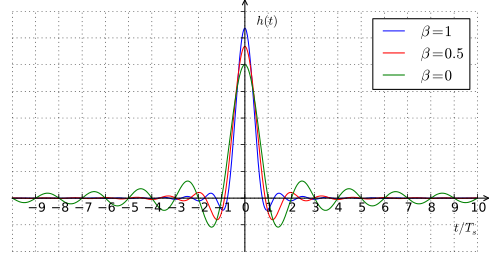
\includegraphics[scale=1]{Imagenes/Factor.png}
	\label{fig:Factor}
		\captionsetup{justification=raggedright,font={scriptsize,bf,it}}
	\caption*{fuente: Wikipedia}
\end{figure}

En su forma discreta la respuesta al impulso del filtro RRC se traduce a la siguiente forma: 

\begin{equation} \label{capcuatro_treinta}
 		 h[n]=\begin{cases}
 		 \frac{1}{Sps}(1+\alpha (\frac{4}{\pi}-1)) & \text{ , } n=0 \\ \\ 
 		 \frac{\alpha}{Sps\sqrt{2}}[(1+ \frac{2}{\pi})sin(\frac{\pi}{4 \alpha})+(1- \frac{2}{\pi})cos(\frac{\pi}{4 \alpha})] & \text{ , } n=  \pm \frac{Sps}{4 \alpha}\\ \\ 
 		 \frac{1}{Sps}\frac{sin[ \pi \frac{n}{Sps}(1- \alpha )]+4 \alpha \frac{n}{Sps}cos[ \pi \frac{n}{Sps}(1+\alpha)]}{ \pi \frac{n}{Sps}[1-(4\alpha\frac{n}{Sps})^2]} & \text{ , } n=otros 
 		 \end{cases}
\end{equation}


\subsubsection{Forma de los pulsos en las Redes Fast Ethernet}

El el sitio web del libro se tiene un víde que muestra cómo se usa este concepto en las redes Fast Ethernet. Este es el enlace directo:
\begin{center}
\url{https://sites.google.com/saber.uis.edu.co/comdig/wf} 
\end{center}

\subsection{Clock Recovery o Timing}

Ya sabemos que, para la recepción de un bit o un símbolo digital, usualmente existe un instante, dentro de ese bit o símbolo que es el más óptimo para analizar qué es lo que viene viajando allí. Eso se ha tratado en el tema de acoplamiento y regeneración de bits o símbolos. El problema que ahora surge consiste en lo siguiente: los fenómenos de propagación dificultan enormemente el timing ya que el instante óptimo no será fijo en la señal de entrada, sino que estará variando en el tiempo. Podemos imaginar esto como una fila de hormigas que intentan llegar a su destino manteniendo una misma distancia entre ellas, pero por cuestiones imprevisibles esa distancia varía, pero posible implementar una especie de peaje donde cada hormiga es separada para que entren a la cueva conservando una misma distancia. \\

La solución se conoce como Timing o Time recovery o clock syncronization, que básicamente consiste en lograr, de manera automática, seleccionar el mejor instante de muestreo de la señal digital recibida en un USRP, aun cuando se estén presentando variaciones de tiempo para ese instante. Esto equivale también a seleccionar la muestra donde el diagrama de ojo aparece más abierto. Pero la tarea va más allá de un Diagrama de Ojo, pues en la mayoría de los casos, el mejor instante para el muestreo no se encuentra ni siquiera entre las muestras de la señal discreta recibida. Es decir, en el proceso de muestreo, que se realiza previo al timing, es posible que el mejor instante de muestreo no sea captado por una de las muestras. Así, por ejemplo, en la siguiente figura, en la parte izquierda, el mejor instante de muestreo es parte de las muestras, pero en la parte derecha no lo es. \\

\begin{figure}[h!]
	\captionsetup{justification = raggedright, singlelinecheck = false}
	\caption{Timing} 
	\centering
	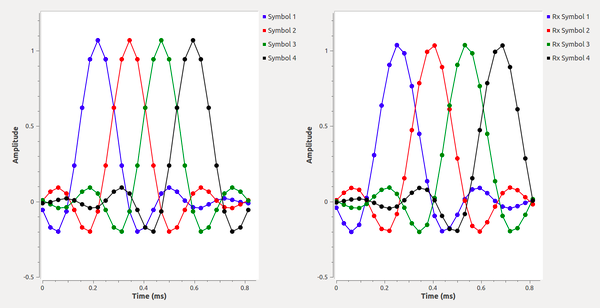
\includegraphics[scale=1]{Imagenes/Simbolo.png}
	\label{fig:Simbolo}
	%	\captionsetup{justification=raggedright,font={scriptsize,bf,it}}
	%	\caption*{fuente: \textcolor{
	%			Orange}{Tomada de Wikipedia}}
\end{figure}

Hay varios algoritmos que podemos utilizar para recuperar el reloj en el receptor, y casi todos ellos implican algún tipo de bucle de control con retroalimentación. Otros se apoyan generalmente en una palabra conocida como un preámbulo. \\

El bloque Polyphase Clock Sync, usa una técnica de recuperación de reloj de filtrado polifásico que se describe en el libro de Fred Harris . Este bloque nos brinda tres cosas: En primer lugar, realiza la recuperación del reloj, en segundo lugar, realiza el acoplamiento entre señal transmitida y recibida para luchar con el problema de ISI. \\

Para usar el bloque se supone que en el transmisor se empleado un Filtro Raíz del Coseno Alzado (Filtro RCC). El principio de funcionamiento consiste en hacer pasar la señal por otro Filtro Raíz de Coseno Alzado para realizar el acoplamiento y luego calcular la primera diferencia de la señal resultante para relacionarla con su desplazamiento del reloj. Como se muestra en la figura siguiente todo parece perfecto en este caso, pues el instante óptimo se encuentra dentro de las muestras recibidas. El filtro de diferencia ([-1, 0, 1]) genera el diferencial del símbolo, y como muestra la siguiente figura, la salida de este filtro en el punto de muestreo correcto es 0. Podemos entonces invertir esa afirmación y en su lugar decir que cuando La salida del filtro diferencial es 0, hemos encontrado el punto de muestreo óptimo. \\

%\vspace{200px}
\begin{figure}[h!]
	\captionsetup{justification = raggedright, singlelinecheck = false}
	\caption{Punto óptimo} 
	\centering
	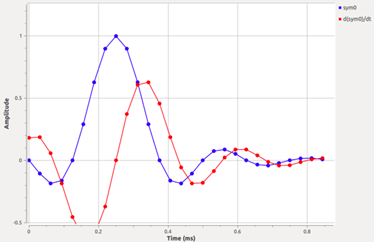
\includegraphics[scale=1.2]{Imagenes/Punto-optimo.png}
	\label{fig:Punto-optimo}
	%	\captionsetup{justification=raggedright,font={scriptsize,bf,it}}
	%	\caption*{fuente: \textcolor{
	%			Orange}{Tomada de Wikipedia}}
\end{figure}

El problema es mayor cuando el punto óptimo no aparece dentro de las muestras recibidas, como se muestra en la siguiente figura. \\

%\vspace{200px}
\begin{figure}[h!]
	\captionsetup{justification = raggedright, singlelinecheck = false}
	\caption{Punto óptimo no aparece dentro de las muestras recibidas} 
	\centering
	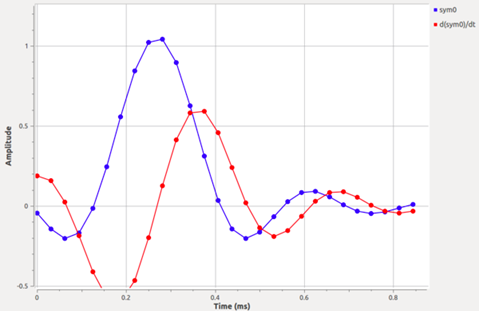
\includegraphics[scale=0.8]{Imagenes/Punto-no-optimo.png}
	\label{fig:Punto-no-optimo}
	%	\captionsetup{justification=raggedright,font={scriptsize,bf,it}}
	%	\caption*{fuente: \textcolor{
	%			Orange}{Tomada de Wikipedia}}
\end{figure}

Por esta razón, el bloque Polyphase Clock Sync usa un número mayor de filtros cada uno con un desfase diferente. Si se tienen suficientes filtros con diferentes desfases, uno de ellos dará el valor del timing que buscamos. En la siguiente figura se muestra el resultado de incluir 5 filtros, lo que significa 5 desfases diferentes y podemos ver que la señal etiquetada como d (sym0) / dt + phi3 tiene un punto de muestreo exactamente igual a 0. Esto nos indica que nuestro punto de muestreo ideal se produce con este desfase. Por lo tanto, si tomamos un filtro RRC de nuestro receptor y ajustamos su fase phi3 (que es $3 * 2\pi / 5$), entonces podemos corregir la falta de sincronización y seleccionar el punto de muestreo ideal para este caso. \\

%\vspace{200px}
\begin{figure}[h!]
	\captionsetup{justification = raggedright, singlelinecheck = false}
	\caption{Búsqueda del punto óptimo} 
	\centering
	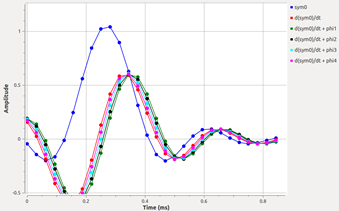
\includegraphics[scale=1.2]{Imagenes/Timing.png}
	\label{fig:Timing}
	%	\captionsetup{justification=raggedright,font={scriptsize,bf,it}}
	%	\caption*{fuente: \textcolor{
	%			Orange}{Tomada de Wikipedia}}
\end{figure}

El resultado del timing en una constelación se ejemplifica en la siguiente figura en la cual se tiene en la parte izquierda la constelación de la señal a la entrada del bloque y en la parte derecha la de la salida. \\

\begin{figure}[h!]
	\captionsetup{justification = raggedright, singlelinecheck = false}
	\caption{Constelación antes y después del timing} 
	\centering
	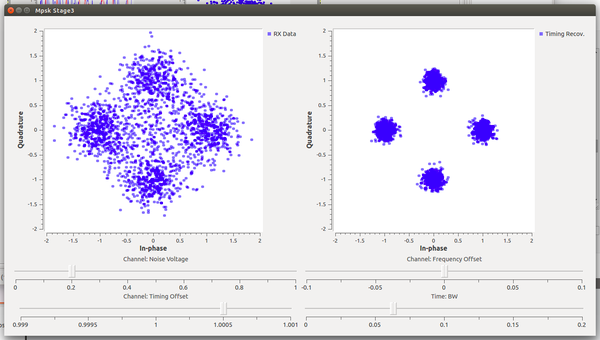
\includegraphics[scale=1]{Imagenes/Resultados-timing.png}
	\label{fig:Resultados-timing}
	%	\captionsetup{justification=raggedright,font={scriptsize,bf,it}}
	%	\caption*{fuente: \textcolor{
	%			Orange}{Tomada de Wikipedia}}
\end{figure}

\subsection{Time alignment}

El problema consiste en que el instante en que comienza un Byte es desconocido para el receptor. Así, por ejemplo, en la siguiente tabla se representan los bytes y los bits que podría estar entregando un transmisor. 
\vspace{200px}
\begin{table}[h!]
	\captionsetup{justification = raggedright,singlelinecheck = false}
	\caption{Alguna descripción.}
	\label{tabla:tabla7}
	\centering
	\scalebox{0.70}{
\begin{tabular}{|c|c|c|c|c|c|c|c|c|c|c|c|c|c|c|c|c|c|c|c|c|c|c|c|c|c|c|c|c|c|c|c|c|}
\hline
Byte & \multicolumn{8}{c|}{23}       & \multicolumn{8}{c|}{56}       & \multicolumn{8}{c|}{1}        & \multicolumn{8}{c|}{99}       \\ \hline
Bits & 0 & 0 & 1 & 0 & 1 & 1 & 1 & 1 & 0 & 0 & 1 & 1 & 1 & 0 & 0 & 0 & 0 & 0 & 0 & 0 & 0 & 0 & 0 & 1 & 0 & 1 & 1 & 0 & 0 & 0 & 1 & 1 \\ \hline
\end{tabular}}
\end{table}



Pero en la siguiente, debido a un retardo que es usualmente desconocido, aunque están llegando los mismos bits, son interpretados como bytes diferentes a los transmitidos. 

\begin{table}[h!]
	\captionsetup{justification = raggedright,singlelinecheck = false}
	\caption{Sin alguna descripción.}
	\label{tabla:tabla8}
	\centering
	\scalebox{0.70}{
\begin{tabular}{|c|c|c|c|c|c|c|c|c|c|c|c|c|c|c|c|c|c|c|c|c|c|c|c|c|c|c|c|c|c|c|c|c|}
\hline
Byte & \multicolumn{8}{c|}{69}       & \multicolumn{8}{c|}{231}      & \multicolumn{8}{c|}{0}        & \multicolumn{8}{c|}{44}       \\ \hline
Bits & 0 & 1 & 0 & 0 & 0 & 1 & 0 & 1 & 1 & 1 & 1 & 0 & 0 & 1 & 1 & 1 & 0 & 0 & 0 & 0 & 0 & 0 & 0 & 0 & 0 & 0 & 1 & 0 & 1 & 1 & 0 & 0 \\ \hline
\end{tabular}}
\end{table}


Como consecuencia, no se obtienen en el receptor los bytes transmitidos a partir de los bits que va recibiendo. \\

Para resolver el problema es posible usar un protocolo superior que permita marcar el comienzo de una emisión o de paquetes de emisión. Esto puede realizarse con un codificador y es lo que se conoce como Time alignment. \\


\subsection{Frequency Lock Loop (FLL) y Phase Local Loop (PLL)}

Un método sencillo para estabilizar una constelación consiste en que el bloque de sincronización tenga la información sobre la constelación usada. Se basa en la implementación de un Bucle de Costas (Costas Loop) para medir la señal recibida en búsqueda del error que presenta con respecto al punto de constelación más cercano en la constelación que se tiene como modelo.  La siguiente figura ha sido tomada de Wikipedia  y refleja muy bien la idea: una señal m(t) puede llegar con una desviación de frecuencias $\varpi$, se involucra un VCO para corregirla.  \\


\begin{figure}[h!]
	\captionsetup{justification = raggedright, singlelinecheck = false}
	\caption{Frequency Lock Loop} 
	\centering
	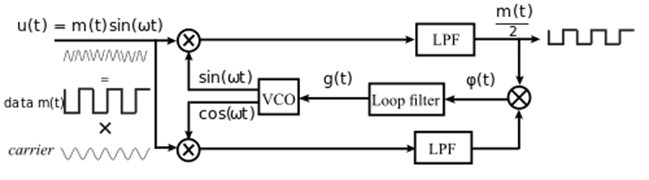
\includegraphics[scale=0.9]{Imagenes/Costas.png}
	\label{fig:Costas}
	\captionsetup{justification=raggedright,font={scriptsize,bf,it}}
	\caption*{fuente:  https://en.wikipedia.org/wiki/Costas-loop}
\end{figure}

De manera similar funciona el FLL (Frequency Lock loop) , pero m(t) es una envolvente compleja. El bloque puede fallar cuando las desviaciones son exageradamente altas. El bloque se conecta usualmente después del ecualizador. \\

Otro bloque es el “Costas Loop”. Este bloque está pensado para ser usados en modulaciones M-PSK, utiliza un bucle de segundo orden y por lo tanto se define con un parámetro de ancho de banda de bucle. La otra cosa que necesita saber es el orden de la modulación M-PSK, de modo que es 2 para BPSK, 4 para QPSK y 8 para 8PSK. En la imagen podemos ver que los símbolos están todos en el círculo de unidad, pero girando debido a que aún no se está realizando aún la compensación de frecuencia. A la salida del bloque de bucle Costas, podemos ver la constelación bloqueada más el ruido extra que no podemos suprimir. \\

\begin{figure}[h!]
	\captionsetup{justification = raggedright, singlelinecheck = false}
	\caption{Antes y después de a plicar FLL} 
	\centering
	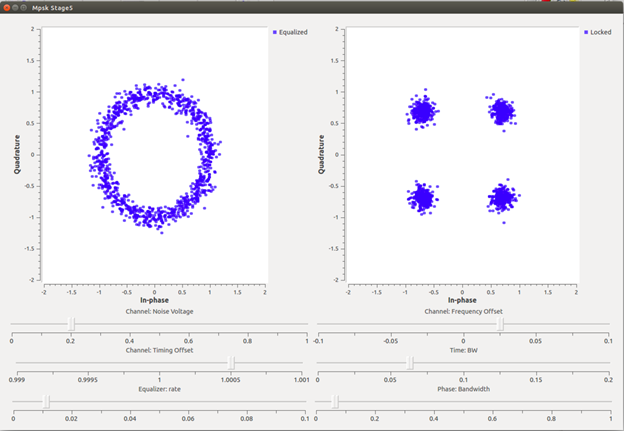
\includegraphics[scale=0.9]{Imagenes/Bucle-costas.png}
	\label{fig:Bucle-costas}
%	\captionsetup{justification=raggedright,font={scriptsize,bf,it}}
%	\caption*{fuente:  https://en.wikipedia.org/wiki/Costas-loop}
\end{figure}

\subsection{La ambigüedad de fase}

Obsérvese que en nuestra discusión anterior la corrección de las desviaciones de frecuencia o de fase se basan en un conocimiento previo de la forma de la constelación, pero debido a que la constelación tiene una forma simétrica es posible que la constelación recibida y procesada resulte girada en un ángulo tal que tenga la misma apariencia de la constelación transmitida. Entonces ocurre que cada punto puede resultar expresando un símbolo diferente al transmitido. Para resolver este problema hay que aprovechar que, en todo caso, se mantiene el orden de la secuencia de los símbolos, es decir, los símbolos siguen llegando en el mismo orden en que fueron emitidos, solo que con fases diferentes. \\

\subsubsection{La codificación diferencial}

La idea es no transmitir los símbolos tal y como se originan sino los que resulten de la diferencia entre ellos, de modo que la información útil no se asocia a un punto de constelación sino a la diferencia entre puntos de constelación. En la parte receptora se obtiene cada símbolo a partir de su relación con otro símbolo adyacente. \\

En la parte transmisora, la solución se implementa mediante un codificador diferencial.Para el caso más sencillo, supongamos que los símbolos transmitidos son simplemente bits y que en un instante determinado, a la entrada del codificador se tiene el bit $x_i$. La salida $y_i$ se calcula así. \\
\begin{equation} \label{capcuatro_treintauno}
	 y_{i} = y_{i-1} \oplus x_i
\end{equation}

Donde $ \oplus$ es la operación de suma binaria o suma por módulo 2. \\ En la parte receptora, se realiza la operación inversa \\
\begin{equation} \label{capcuatro_treintados}
	 x_{i} = y_{i} \oplus y_{i-1}
\end{equation}

De modo que en el receptor el valor de $x_i$ no está en un determinado símbolo $y_i$ sino en la diferencia con respecto al símbolo anterior $y_{i-1}$. \\

Para llevar a cabo esta idea en el caso en que se usan símbolos compuestos por $k$ bits, es necesario aplicar la operación a paquetes de $k$ bits, así, en el caso de BPSK, $k=1$; en QPSK, $k=2$; en 8PSK, $k=3$; en 16QAM, $k=4$. Cabe notar que $k=log_2(M)$, donde $M$ es el número de puntos de constelación de la modulación de interés \\

Veamos un ejemplo para la modulación 8PSK: \\

\begin{itemize}
	\item [$\bullet$] El símbolo actual es $x_i=110$
	\item [$\bullet$] El símbolo anterior era $y_{i-1}=101$
	\item [$\bullet$] La salida del encoder es: $y_i=y_{i-1} \oplus x_i = 101 \oplus 110=011$	
	\item [$\bullet$] En el decoder se realiza la operación: $x_i = y_i  \oplus y_{i-1} = 011 \oplus 101=110 $
\end{itemize}\\

Veamos un ejemplo más completo para la misma modulación:\\

Supongamos que la señal a la entrada del codificador es $110010011100$ y que puede ser ser vista como símbolos de a 3 bits de la siguiente manera:\\

$x=[110] [010] [011] [100]$\\

Supongamos que al iniciar el proceso el codificador está en estado:\\

$y_0=[111]$\\

con la llegada del primer símbolo al codificador se produce la salida de la siguiente manera:\\

$y_1=y_0 \oplus x_1 = 111 \oplus 110=001$\\

con el segundo símbolo\\

$y_2=y_1 \oplus x_2 = 110 \oplus 010=011$\\

Con el tercer símbolo\\

$y_3=y_2 \oplus x_3 = 011 \oplus 011=000$\\

Con el cuarto símbolo\\

$y_4=y_3 \oplus x_4 = 000 \oplus 100=100$\\

Veamos ahora lo que ocurre en la parte receptora\\

Al decodificador llega la señal:\\

$y=[111] [001] [011] [000] [100]$\\

Con la llegada del primer símbolo al decodificador se produce la salida de la siguiente manera:\\

$x_1=y_0 \oplus y_1 =111 \oplus 001=110$\\

con el segundo símbolo\\

$x_2=y_1 \oplus y_2 =001 \oplus 011=010$\\

con el tercer símbolo\\

$x_3=y_2 \oplus y_3 =011 \oplus 000=011$\\

con el cuarto símbolo\\

$x_4=y_3 \oplus y_4 =000 \oplus 100=100$\\

Como podemos ver, la salida del decodificador es: $110010011100$ y es igual a la entrada del codificador.

\subsubsection{La codificación diferencial generalizada}

La operación $y_{i-1} \oplus x_i$ no es la única forma para una codificación diferencial. De manera más genérica, se puede usar una función $u=F(x,y)$ siempre y cuando la ecuación $u_0 = F(y_0,x)$ solo tenga una solución para cualquier $y_0$ y $u_0$. 

\subsubsection{Problemas de la codificación diferencial}

La codificación diferencial tiene una desventaja significativa: multiplica errores. Esto es, si un símbolo $y_i$ es recibido incorrectamente, habrán dos símbolos de información $x_i$ y $x_{i+1}$ decodificados incorrectamente ya que ambos depende de $y_i$, pues: $x_i = y_i \oplus y_{i-1}$, pero $x_{i+1}= y_{i+1} \oplus y_i$ . Por esa razón, la rata de símbolos perdidos se dobla. \\

Existen otras alternativas para para resolver ambigüedad de fase. Por ejemplo, en la televisión digital satelital, con el sistema DVB-S, se usan syncword sobre una trama de sincronización, de manera que si en esa trama se detecta que las syncword están invertidas de alguna manera, todos los datos proceden a ser invertidos de manera consecuente. \\

\subsection{El Control Automático de la Ganancia}
De acuerdo a lo visto, es inevitable que la señal a la salida de USRP receptor esté variando su magnitud de manera impredecible. Un AGC puede permitir estabilizar ese parámetro de una manera aceptable para su observación y procesamiento. El sistema puede ser implementado basado en el sistema retroalimentado de bucle cerrado que aparece en la siguiente figura. 

%\setcounter{figure}{107}
\vspace{200px}
\begin{figure}[h!]
	\captionsetup{justification = raggedright, singlelinecheck = false}
	\caption{Elemento de Área donde puede localizarse el receptor} 
	\centering
	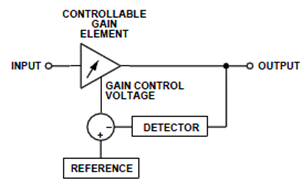
\includegraphics[scale=1]{Imagenes/PLL.png}
	\label{fig:PLL}
	%	\captionsetup{justification=raggedright,font={scriptsize,bf,it}}
	%	\caption*{fuente: \textcolor{
	%			Orange}{Tomada de Wikipedia}}
\end{figure}

Básicamente se cuenta con una referencia, que es el nivel deseado de señal. El detector está midiendo permanentemente el nivel de señal a la salida. La diferencia de los anteriores valores permite regular la ganancia del amplificador. Una descripción más detallada se encuentra en el trabajo de \textcolor{red}{Tom Rondau- REFERENCIAR} quien desarrolló un AGC en gnuradio que se resume en la figura siguiente. \\

\begin{figure}[h!]
	\captionsetup{justification = raggedright, singlelinecheck = false}
	\caption{AGC según Tom Rondau} 
	\centering
	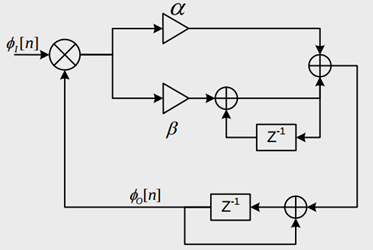
\includegraphics[scale=1]{Imagenes/AGC.png}
	\label{fig:AGC}
	%	\captionsetup{justification=raggedright,font={scriptsize,bf,it}}
	%	\caption*{fuente: \textcolor{
	%			Orange}{Tomada de Wikipedia}}
\end{figure}

El sistema permite realizar un seguimiento continuo del nivel de señal, pero es claro que no contribuye a mejorar la relación señal a ruido. En realidad, todo radio receptor contiene un AGC. \\

\subsection{El Ecualizador}

En muchos casos la señal que pasa por un canal sufre diversas alteraciones en función de la frecuencia. La ecualización del canal busca determinar cuáles son esas alteraciones, intentando descubrir la respuesta en frecuencias del canal para luego sintonizar un filtro con la respuesta en frecuencias inversa para corregir el efecto del canal.

\vspace{200px}
\begin{figure}[h!]
	\captionsetup{justification = raggedright, singlelinecheck = false}
	\caption{Variaciones espectrales del canal (rojo) versus respuesta en frecuencias del Ecualizador} 
	\centering
	\includegraphics[scale=1]{Imagenes/Inversa.png}
	\label{fig:Inversa}
	%	\captionsetup{justification=raggedright,font={scriptsize,bf,it}}
	%	\caption*{fuente: \textcolor{
	%			Orange}{Tomada de Wikipedia}}
\end{figure}

\begin{itemize}
	\item [$\bullet$]\textbf{Filtro digital:} El principal componente de un ecualizador es un simple filtro digital, que no es otra cosa que un sistema Lineal e Invariante en el Tiempo (LIT). De modo que se trata de un sistema que tiene una respuesta al impulso h[n], una entrada x[n] y una salida y[n], como el de la siguiente figura. \\
	
%	\vspace{200px}
	\begin{figure}[h!]
		\captionsetup{justification = raggedright, singlelinecheck = false}
		\caption{Sistema LIT} 
		\centering
		\includegraphics[scale=1]{Imagenes/Diagrama-trans.png}
		\label{fig:Diagrama-trans}
		%	\captionsetup{justification=raggedright,font={scriptsize,bf,it}}
		%	\caption*{fuente: \textcolor{
		%			Orange}{Tomada de Wikipedia}}
	\end{figure}

\begin{equation} \label{capcuatro_treintatres}
	 y[n]= x[n]*h[n]
\end{equation}

En los sistemas reales, como es el caso de GNU Radio, $h[n]$ es un conjunto de valores $W_k$ cada uno de los cuales representa el valor de amplitud de la muestra k de $h[n]$, como se muestra en la siguiente figura. \\

\begin{figure}[h!]
	\captionsetup{justification = raggedright, singlelinecheck = false}
	\caption{Respuesta al impulso de un Ecualizador} 
	\centering
	\includegraphics[scale=1]{Imagenes/Muestras.png}
	\label{fig:Muestras}
	%	\captionsetup{justification=raggedright,font={scriptsize,bf,it}}
	%	\caption*{fuente: \textcolor{
	%			Orange}{Tomada de Wikipedia}}
\end{figure}

De modo que podemos, aplicando el concepto de convolución, decir que.\\

\begin{equation} \label{capcuatro_treintacuatro}
	 y[n]=w[k]*x[n]= \sum_{k=1}^{p}w_{k} x[n-kl] \\
\end{equation}
	
En GNU Radio se tienen bloques que juegan el papel de filtro digital, para lo cual hay que configurarle un vector w que contiene los pesos $W_k$. Esos pesos se conocen en GNU Radio como taps.\\

	\item [$\bullet$] \textbf{El Ecualizador fijo:} Un filtro como el anterior, con una respuesta al impulso adecuada, podría resolver la necesidad de ecualización del canal. \\

%	\vspace{200px}	
	\begin{figure}[h!]
		\captionsetup{justification = raggedright, singlelinecheck = false}
		\caption{Proceso de entrenamiento del ecualizador} 
		\centering
		\includegraphics[scale=1]{Imagenes/Ecualizador.png}
		\label{fig:Ecualizador}
		%	\captionsetup{justification=raggedright,font={scriptsize,bf,it}}
		%	\caption*{fuente: \textcolor{
		%			Orange}{Tomada de Wikipedia}}
	\end{figure}

\vspace{300px}
	
	\begin{figure}[h!]
	\captionsetup{justification = raggedright, singlelinecheck = false}
	\caption{El ecualizador funcionando con pesos obtenidos durante el entrenamiento} 
	\centering
	\includegraphics[scale=1]{Imagenes/Ecualizador-dos.png}
	\label{fig:Ecualizador-dos}
	%	\captionsetup{justification=raggedright,font={scriptsize,bf,it}}
	%	\caption*{fuente: \textcolor{
	%			Orange}{Tomada de Wikipedia}}
\end{figure}


	\item [$\bullet$] \textbf{El Ecualizador adaptativo}

	\begin{figure}[h!]
		\captionsetup{justification = raggedright, singlelinecheck = false}
		\caption{Ecualización adaptativo} 
		\centering
		\includegraphics[scale=1]{Imagenes/Ecualizador-adaptativo.png}
		\label{fig:Ecualizador-adaptativo}
		%	\captionsetup{justification=raggedright,font={scriptsize,bf,it}}
		%	\caption*{fuente: \textcolor{
		%			Orange}{Tomada de Wikipedia}}
	\end{figure}

\vspace{300px}

	\begin{figure}[h!]
	\captionsetup{justification = raggedright, singlelinecheck = false}
	\caption{Respuesta variante al Impulso de un Ecualizador} 
	\centering
	\includegraphics[scale=1]{Imagenes/Pesos.png}
	\label{fig:Pesos}
	%	\captionsetup{justification=raggedright,font={scriptsize,bf,it}}
	%	\caption*{fuente: \textcolor{
	%			Orange}{Tomada de Wikipedia}}
	\end{figure}

	\item [$\bullet$]\textbf{Filtro basado en los mínimos cuadrados medios (LMS). Filtro de Wiener y Hopf o Filtro LMS:}
	
	Los problemas a resolver son dos: el de obtener esa respuesta al impulso adecuadas y el de recalcularla cada vez que el canal cambie de estado.  Esto se logra, si el filtro digital es complementado con un Algoritmo que estudie lo que se espera de él para recalcular los pesos o taps del filtro. Es necesario informar a este filtro lo que de él se espera y esto se puede realizar mediante una señal de error.
	
	\begin{figure}[h!]
		\captionsetup{justification = raggedright, singlelinecheck = false}
		\caption{Filtro adaptativo} 
		\centering
		\includegraphics[scale=1]{Imagenes/Filtro-adaptativo.png}
		\label{fig:Filtro-adaptativo}
		%	\captionsetup{justification=raggedright,font={scriptsize,bf,it}}
		%	\caption*{fuente: \textcolor{
		%			Orange}{Tomada de Wikipedia}}
	\end{figure}

Ahora es tiempo de preguntarnos qué operaciones realiza el Algoritmo Adaptativo. El algoritmo deberá seleccionar valores para el vector w y analizar cómo ellos van influyendo en el error e[n] para hasta lograr que la media cuadrática del error sea la mínima posible. De esta manera, el índice de desempeño elegido es el valor cuadrático medio.\\

\begin{equation} \label{capcuatro_treintacinco}
	 J=E[(d[n]-y[n])^{2}]
\end{equation}

El criterio para encontrar los pesos consiste en lograr que ese índice de desempeño sea el mínimo, con lo cual llegamos a aplicar el criterio de aproximación conocido como el mínimo de la media cuadrada o LMS (Least Mean Square).\\

\begin{equation} \label{capcuatro_treintasies}
	J=Jmin
\end{equation}

Como d[n] es la señal que se desea a la salida del filtro, entonces puede decirse que se desea que. \\

\begin{equation} \label{capcuatro_treintasiete}
	y[n]= \sum_{k=1}^{p}=  w_{k}x[n-kl]
\end{equation}

Por lo tanto se desea que

\begin{equation} \label{capcuatro_treintaocho}
	J= E \left([d[n]-\sum_{k=1}^{p}=  w_{k}x[n-kl]]\right)^{2}
\end{equation}

Desenvolviendo lo anterior, teniendo en cuenta que: \\


\begin{equation} \label{capcuatro_treintanueve}
	\sum_{k=1}^{2}a_{k} * \sum_{k=1}^{2}a_{j} = \sum_{k=1}^{2}\sum_{k=1}^{2}a_{k}a_{j}
\end{equation}



obtenemos. \\

\begin{equation} \label{capcuatro_cuarenta}
	J= E [d^{2}[n]]-2  \sum_{k=1}^{p}w_{k}E [d[n]x[n-k]]+ \sum_{j=1}^{p} \sum_{k=1}^{p} w_{j} w_{k} E[x[n-j]x[n-k]]
\end{equation}
\end{itemize}

Se pueden realizar algunas simplificaciones si se tiene en cuenta que: \\

\begin{itemize}
	\item [$\bullet$] La señal x(t) es la función muestra de un proceso estacionario X(t) y su versión muestreada x[n] tiene media. \\
	
	\begin{equation} \label{capcuatro_cuarentayuno}
		\mu_{X}[n] = \mu_{X}= 0= E[x[n]]
	\end{equation} 
\item [$\bullet$] De lo anterior se deduce que la varianza. \\

	\begin{equation} \label{capcuatro_cuarentaydos}
	E[(x[n]- \mu_{x})^{2}] = E[x^{2}[n]] = \sigma_{x}^{2} 
	\end{equation} 	
	
\item [$\bullet$] Sabiendo que la función de autocorrelación está definida como: 

	\begin{equation} \label{capcuatro_cuarentaytres}
	 E[x[n]x[n-k]]=R_X[k]
	\end{equation} 
\item [$\bullet$] y que la función de cross correlación entre $d[n]$ y $x[n]$ es: \\

	\begin{equation} \label{capcuatro_cuarentaycuatro}
	 E[d[n]x[n-k]]=R_{DX}[k]
\end{equation} 

Se deduce que: \\

\begin{equation} \label{capcuatro_cuarentaycinco}
	 J= \sigma_{x}^{2}-2 \sum_{k=1}^{p} w_{k} R_{DX}[k]+\sum_{j=1}^{p} \sum_{k=1}^{p} w_{j} w_{k}R_{X}[k-j]
\end{equation}

Lo que resta es identificar qué pasa con los pesos w cuando $J=J_{min}$, con lo cual podríamos llegar a despejar los pesos óptimos $w_{o}$, como se muestra en la siguiente figura. \\


\begin{figure}[h!]
	\captionsetup{justification = raggedright, singlelinecheck = false}
	\caption{El mínimo de la media cuadrática } 
	\centering
	\includegraphics[scale=1]{Imagenes/Jmin.png}
	\label{fig:Jmin}
	%	\captionsetup{justification=raggedright,font={scriptsize,bf,it}}
	%	\caption*{fuente: \textcolor{
	%			Orange}{Tomada de Wikipedia}}
\end{figure}
\end{itemize}

El mínimo error cuadrático medio Jmin  se presenta cuando el gradiente (la pendiente) del error cuadrático medio J es cero. De modo que si nos interesa hallar $W_k=W_{0k}$ para ese caso, debemos despejar $W_k$ cuando $ \dfrac{ \delta J}{ \delta W_{k}}= 0$. \\

\begin{equation} \label{capcuatro_cuarentayseis}
	g_k = \dfrac{ \delta J}{ \delta W_{k}}= -2R_{DX}[k]+2 \sum_{k=1}^{p} w_j R_{X}[k-j]
\end{equation}

Igualando a cero el vector gradiente $g_k$, se obtiene la Expresión de optimización de los Mínimos Cuadrados de Wiener-Hopf, también conocida como Ecuaciones de Wiener Hopf: \\

\begin{equation} \label{capcuatro_cuarentaysiete}
	 R_{DX}[k] = \sum_{j=1}^{p} w_j R_X [k-j]
\end{equation}

Veamos el conjunto de todos los valores que intervienen en esta ecuación. Ellos se pueden organizar en forma matricial. \\

\begin{equation} \label{capcuatro_cuarentayocho}
	 r_{DX}= \left[
	 \begin{array}{c}
     R_{DX}[1]\\
     R_{DX}[2]\\
     .\\
     .\\
     .\\
     R_{DX}[p]
     \end{array}
     \right];
     w_{0}= \left[
	 \begin{array}{c}
     w_{1}\\
     w_{2}\\
     .\\
     .\\
     .\\
     w_{p}
     \end{array}
     \right];
\end{equation}

\begin{equation} \label{capcuatro_cuarentaynueve}
	 R_X= \left[
	 \begin{array}{cccc}
     R_X[0] & R_X[1] & ... & R_X[p-1]\\
     R_X[1] & R_X[0] & ... & R_X[p-2]\\
     .\\
     .\\
     .\\
     R_X[p-1] & R_X[p-2] & ... & R_X[0]
     \end{array}
     \right]
\end{equation}
\\
$R_X$ es conocida como la matriz simétrica de Toepliz. Representando $R_X$ y $w_0$ de la forma vectorial siguiente:

\begin{equation} \label{capcuatro_cincuenta}
w_{0} = [w_1 , w_2, ... , w_p]^{T} \\
r_{DX} = [R_{DX}[1], R_{DX}[2], ... , R_{Dx}[p]]^{T}   \\
\end{equation}

Se obtiene la forma matricial de la expresión de optimización.

\begin{equation} \label{capcuatro_cincuentayuno}
	 r_{DX}=w_oR_X
\end{equation}

Facilitando el despeje de los pesos así: \\

\begin{equation} \label{capcuatro_cincuentaydos}
	 w_{o}= r_{DX}R_{X}^{-1}
\end{equation}

$R_X^{-1}$ es la inversa de $R_X$ y se supone que existe pues $R_X$ no es singular.

\begin{itemize}
	\item [$\bullet$] \textbf{Filtro Recursivo basado en los mínimos cuadrados medios (RLS)} \\
	
	Se trata del mismo Filtro LMS solo que se usa un método conocido como el descenso más pronunciado (deepest descent) para obtener una ecuación donde los pesos pueden ser hallados de manera recurrente, realizando un ligero ajuste a los pesos previamente calculados. \\
	
	\begin{equation} \label{capcuatro_cincuentaytres}
		 w_k [n+1]=w_k[n]+x[n-k] e[n], k=0,1,...,N
    \end{equation}

$ \mu$ Es un paso que el algoritmo usa para ir buscando el valor $Jmin-ideal$ a partir de un valor $Jmin-ya-calculado$.
Este es quizá el método más utilizado en ecualización adaptativa. A continuación algunos apuntes sobre experiencias de trabajo con este tipo de filtros:

\begin{itemize}
	\item [$\bullet$] En cuanto mayor sea el parámetro del tamaño del escalón $\mu$, tanto más rápida la capacidad de rastreo del ecualizador adaptable.
	\item [$\bullet$] Un parámetro grande de $\mu$   quizá resulte en un error cuadrático medio de exceso inaceptablemente alto, es decir, excede exageradamente a Jmin
	\item [$\bullet$] Entre más pequeño sea m encontramos que después de un gran número de interacciones el comportamiento del algoritmo de Mínimos Cuadrados es casi similar al del Algoritmo de Descenso Pronunciado, que utiliza el gradiente real en vez de la estimación de error para el cálculo de los pesos del filtro
	\item [$\bullet$] La elección en la práctica de un valor adecuado para $\mu$ implica establecer un compromiso entre el rastreo rápido y la reducción del error cuadrático medio de exceso
	\item [$\bullet$] El bloque LMS de Simulink tiene una opción para usar una forma normalizada del algoritmo LMS para que  resulte limitada así: $0<\mu <2$	
\end{itemize}
\end{itemize}

Proceso que realiza el filtro: \\

1.En cada paso se halla un nuevo $Jmin-ya-calculado=Jmin-calculado+ \mu$. \\

2.luego analiza la diferencia con el $Jmin-ideal$. \\

3.si no alcanza este $Jmin-ideal$, entonces vuelve al punto 1. \\

Para el caso, cuando no se usa el algoritmo normalizado,  \textcolor{blue}{\href{https://drive.google.com/file/d/1XoqU-Hh8m18M3muvptJiY-LHh5bgdcwV/view?usp=sharing}{el material “Ecualización adaptativa de un canal digital ” del profesor Lorenzo Díaz}} es el màs explícito encontrado hasta ahora. \\

El profesor Lorenzo afirma que es muy difícil encontrar el valor óptimo de $ \mu$ en tiempo real, pero que hay una manera aproximada y rápida: \\

\begin{equation} \label{capcuatro_cincuentaycuatro}
	 0 < \mu <\dfrac{2}{3LP_{X}}
\end{equation}

Donde L: es el tamaño del filtro, es decir el tamaño del vector de pesos y $P_{x}$: la potencia media de la señal


\subsection{la Ecualización en GNU Radio}
	
GNU Radio viene con dos ecualizadores fácilmente utilizables. El ecualizador de CMA Equalizer y el LMS DD Equalizer. El CMA, o Algoritmo de Módulo Constante, es un ecualizador ciego, porque no necesita mucha información sobre la señal originalmente transmitida, pero sólo funciona con señales que tienen una amplitud constante, o módulo, como es el caso de la modulación M-PSK ya que los puntos de constelación están en un círculo. El algoritmo de CMA acepta el número de taps a utilizar en el ecualizador, que se basará en una combinación de una conjetura educada, las mejores prácticas conocidas y quizás algún conocimiento real del canal en sí. \\

La siguiente figura ha sido obtenida al conectar un bloque CMA Equalizar de 11 taps a la salida de un Polyphase Clock Sync. La constelación y el espectro a la izquierda corresponden a la entrada del Ecualizador, las de la derecha a la salida. \\

El “LMS DD Equalizer” usa un filtro de predicción basado en el principio del mínimo error medio cuadrático (Least Mean Square) con decisión directa (DD) con respecto a una información que se conoce sobre la señal originalmente transmitida. En el caso del bloque usado en GNU Radio, lo que se conoce de la señal originalmente transmitida en la forma de la constelación. El filtro va recalculando los taps del filtro vigilando que la salida corresponda con la constelación que se tiene como modelo. Puede fallar cuando SNR es demasiado alta, arruinando el desempeño. Este bloque además tiene mayor complejidad computacional. \\

\vspace{300px}
\begin{figure}[h!]
	\captionsetup{justification = raggedright, singlelinecheck = false}
	\caption{Resultado del la Ecualización. A la izquierda sin ecualización. A la derecha con Ecualización} 
	\centering
	\includegraphics[scale=1]{Imagenes/Flujograma-gnu.png}
	\label{fig:Flujograma-gnu}
%		\captionsetup{justification=raggedright,font=%{scriptsize,bf,it}}
%	\caption*{fuente: \textcolor{
%				Orange}{Tomada de https://wiki.gnuradio.org/index.php/Guided-Tutorial-PSK-Demodulation7.7.-Multipath}}
\end{figure}


\section{Ejercicios resueltos}
\subsection{Ejercicio 1.}
\subsubsection{Enunciado}
Se quiere enviar una señal de audio muestreada con una frecuencia de $22[kHz]$. Internamente se usa modulación PCM, previa cuantificación de 8 [bits/muestra] con una amplitud máxima de $0,6[V]$ y símbolos que se entregan a la razón de 4 muestras cada uno al USRP.\\
Implementar el flujograma paso a paso para emitir usando modulación BPSK y realizar los cálculos que sean necesarios.
\subsubsection{Respuesta}
\begin{itemize}

\item \textbf{PARTE I}\\
% \justify 
Para aplicar la modulación PCM se requiere previamente obtener la señal debidamente muestreada y cuantificada, para lo cual estamos usando un bloque construido especialmente para ello $b\_quantizer\_fb$ en el entorno de GNU Radio, como se muestra en la Figura \ref{fig:ej1_pcm_flujo}. Allí, las muestras de la señal con valores numéricos decimales son discretizados en amplitud según la cantidad de niveles de amplitud con que se quiera representar cada una de las muestras a la salida de ese cuantificador. Para nuestro caso, usaremos $2^{Nbps} = 256$ niveles de cuantificación. Enseguida viene la capa que aplica propiamente la modulación PCM, es decir, la capa entre entrega la señal en forma de UNOS y CEROS. La señal PCM se obtiene mediante el bloque "Unpack K Bits", como se muestra en la Figura \ref{fig:ej1_pcm_flujo} el cual simplemente desempaqueta los unos y los ceros que componen a los valores de amplitud de las muestras que entrega el cuantificador. Para nuestro caso, tenemos 256 niveles de amplitud, lo cual equivale a 8 bits por muestra. En la Figura \ref{fig:ej1_pcm_t} se observa parte de la señal PCM, a la salida del bloque "Unpack K Bits".  

\begin{figure}[h!]
	\captionsetup{justification = raggedright, singlelinecheck = false}
	\caption{Flujograma hasta la capa PCM.} 
	\centering
	\includegraphics[scale=0.5]{Imagenes/T6.png}
	\label{fig:ej1_pcm_flujo}
%		\captionsetup{justification=raggedright,font=%{scriptsize,bf,it}}
%	\caption*{fuente: \textcolor{
%				Orange}{Tomada de https://wiki.gnuradio.org/index.php/Guided-Tutorial-PSK-Demodulation7.7.-Multipath}}
\end{figure}


Los siguientes son los cálculos a realizar. Se tiene que el $samp \_rate\_audio$ es 22kHz, el Nbps es 8 y el vp 0.6V, a partir de esto calcule el número de niveles del cuantizador (NivelesQ) y el voltaje máximo (Vmax).
A continuación se presentan las ecuaciones finales necesarias para completar el flujograma con el que se estudiarán las gráficas vistas desde la capa PCM, tanto en tiempo como en frecuencia.

\begin{equation} \label{capcuatro_cincuentaycinco}
samp\_rate\_audio=22kHz \\
\end{equation}

\begin{equation} \label{capcuatro_cincuentayseis}
Nbps = 8 \\
\end{equation}

\begin{equation} \label{capcuatro_cincuentaysiete}
NivelesQ = 2^{Nbps} = 256\\
\end{equation}

\begin{equation} \label{capcuatro_cincuentayocho}
V_{p}= 0.6v\\
\end{equation}

\begin{equation} \label{capcuatro_cincuentaynueve}
Vmax = V_{p}=0.6 v\\
\end{equation}

\vspace{200px}
\begin{figure}[h!]
    \captionsetup{justification = raggedright, singlelinecheck = false}
    \caption{Gráfica en el tiempo en capa PCM
    \label{fig:ej1_pcm_t}
    \textcolor{red}{Error: hay dos curvas, la azul y la roja. la azul parece mal o sobra. Al actualizar se puede aprovechar para hacer las gráficas más nítidas}}
    \includegraphics[width=0.7\linewidth]{Imagenes/tiempocapa6.png}
    \centering
\end{figure}

La siguiente pregunta es: ¿Cuál sería la duración de cada bit?\\

\begin{equation} \label{capcuatro_sesenta}
T_{b}=1/R_{b} = 1/R_{s}
\end{equation}

\begin{equation} \label{capcuatro_sesentayuno}
R_{b}= Nbps X samp\_rate\_audio =176kbps
\end{equation}

\begin{equation} \label{capcuatro_sesentaydos}
T{b}= 5.681us
\end{equation}


La frecuencia de muestreo hasta este punto es igual a Rb porque hay solo una muestra por cada bit.\\

\begin{equation} \label{capcuatro_sesentaytres}
s(t) = \sqrt{\dfrac{2E_{b}}{T_{b}}} Cos(2\pi f_{c}t+ \pi (1-n)) 
\end{equation}

Como se observa en la ecuación \ref{capcuatro_sesentaytres} la PSD corresponde a la de una señal de ruido blanco, pero presenta un delta en $0 Hz$. El delta es debido a que la señal de la Figura \ref{fig:ej1_pcm_t} tiene un nivel de DC, debido a que ella oscila entre 0 y 1. Quizá los lectores esperarían que la PSD tuviese la forma de una función sinc() o algo parecido. Sin embargo no es así debido a que la señal binaria no está aún siendo representada mediante formas rectangulares.

\item \textbf{PARTE II}\\

Para esta nueva capa queremos que nuestra señal sea bipolar con el fin de aproximarnos a la forma de una señal con modulación BPSK bandabase. Previamente usamos el bloque Scrambling para lograr que la PSD sea realmente plana, como se ha explicado en la parte teórica. \\
Lo que sigue es la implementación del modulador BPSK en bandabase. Lo hacemos con los bloques float to complex y null source, como ya se ha explicado en la parte teórica. La implementación se muestra en la Figura \ref{fig:ej1_bpsk_flujo}\\

\vspace{200px}
\begin{figure}[h!]
	\captionsetup{justification = raggedright, singlelinecheck = false}
	\caption{Flujograma de la capa que incluye el Scrambling}
	\label{fig:ej1_bpsk_flujo}
    \includegraphics[width=0.6\linewidth]{Imagenes/T4_T5_parte1.png}
    \centering
\end{figure}

La descripción matemática de una señal modulada BPSK es la siguiente:

\begin{equation}  \label{capcuatro_sesentaycuatro}
	s(t)=	\sqrt{\frac{2E_{b}}{T_{b}}}cos(2\pi f_{c} t+\pi (1-n))	
\end{equation}

Donde $n \in \{0,1\}$. Se supone $n$que toma el valor 0 o el valor 1 dependiendo de la información binaria que la señal debe llevar. Esta expresión proporciona dos fases: $0\deg$ y $180\deg$ ($\pi$ radianes). En la forma específica, los datos binarios se transmiten a menudo con las siguientes señales:


\begin{equation} \label{capcuatro_sesentaycinco}
	s_0(t)=	\sqrt{\frac{2E_b}{T_b}}cos(2\pi f_c t+\pi)=-\sqrt{\frac{2E_b}{T_b}}cos(2\pi f_c t)			
\end{equation}

\begin{equation} \label{capcuatro_sesentayseis}
	s_1(t)=	\sqrt{\frac{2E_b}{T_b}}cos(2\pi f_c t)			
\end{equation}

$f_c$: frecuencia de la onda portadora.\\
$s_0(t)$: señal de salida para el "0" lógico.\\
$s_1(t)$: señal de salida para el "1" lógico.\\

\vspace{300px}
\begin{figure}[h!]
	\captionsetup{justification = raggedright, singlelinecheck = false}
	\caption{Flujograma de la capa BPSK bandabase}
	\label{fig:ej1_bpsk_flujo2}
    \includegraphics[width=0.6\linewidth]{Imagenes/T4_T5_parte2.png}
    \centering
\end{figure}

\textcolor{Red}{Aplicando la Conversión RF (\ref{equ_rfc}):}

\begin{equation} \label{capcuatro_sesentaysiete}
s_ec(t)=\begin{Bmatrix}
 & e^{j0} \rightarrow  unos \\ 
 & e^{j\pi}\rightarrow ceros
\end{Bmatrix}
\end{equation}

\begin{equation} \label{capcuatro_sesentayocho}
s_ec(t)=\begin{Bmatrix}
 & 1 \rightarrow  unos \\ 
 & -1\rightarrow ceros
\end{Bmatrix}
\end{equation}

La envolvente compleja es la misma señal binaria bipolar compleja, pero con parte imaginaria igual a cero.


\begin{figure}[h!]
	\captionsetup{justification = raggedright, singlelinecheck = false}
	\caption{Gráfica PSD después del Scrambling} 
	\centering
	\includegraphics[scale=0.4]{Imagenes/capa5.png}
	\label{fig:ej1_psd_scram}
	%		\captionsetup{justification=raggedright,font={scriptsize,bf,it}}
	%		\caption*{fuente: http://superkuh.com/rtlsdr.html}
\end{figure}

Para BPSK tenemos que0 $R_{s}=R_{b}$,ya que en este punto se esta hablando de símbolos y por lo tanto la frecuencia de muestreo es igual a Rs. \\

\begin{figure}[h!]
	\captionsetup{justification = raggedright, singlelinecheck = false}
	\caption{Gráfica de las señal binaria discreta luego del scrambling}
	\label{fig:ej1_scram_t}
   \includegraphics[width=0.8\linewidth]{Imagenes/tiempocapa5.png}
   \centering
\end{figure}

En la Figura \ref{fig:ej1_psd_scram} y \ref{fig:ej1_scram_t} se muestra el resultado de la operación de Scrambling.\\


En la capa de modulación podemos ver  a la salida una señal parecida a la Figura \ref{fig:ej1_scram_t}. pero ahora pertenece al mundo complejo puesto que a partir del \textit{Float to Complex} se encuentra compuesta de parte Real e Imaginaria. \\

\item \textbf{PARTE III}\\

Para profundizar definiremos los dos bloques nuevos:\\
\ \\ %
El bloque de \textit{Zero order hold} es un retenedor de orden cero. De modo que cada muestra la repite Sps veces, donde Sps es el tiempo discreto de retención. Usaremos este bloque para que los símbolos parezcan tener forma rectangular, es la operación que se conoce como Wave Forming. \\
\ \\ %
El bloque  \textit{b-sampler-cc} el cual recibe una señal y la entrega en forma diezmada por la salida superior, lo cual equivale a una especie de muestreo aplicado a una señal discreta. Lo que se busca es revertir el proceso de Wave Forming, de modo que en ese diezmado se elimian periódicamente un grupo de Sps muestras, con lo cual disminuye Sps la frecuencia de  muestreo.\\

\begin{equation} \label{capcuatro_sesentaynueve}
 sea, Sps=4
\end{equation}

\vspace{200px}
\begin{figure}[h!]
	\captionsetup{justification = raggedright, singlelinecheck = false}
    \caption{Flujograma para la capa de precanal}
    \label{fig:ej1_precanal_flujo}
    \includegraphics[width=0.7\linewidth]{Imagenes/r.png}
    \centering
\end{figure}

El el bloque  \textit{Noise Source}. Se ha implementado para realizar una simulación de la recepción de una señal de audio del mundo real para lo cual  agrega una componente de ruido gaussiano.

\begin{figure}[h!]
	\captionsetup{justification = raggedright, singlelinecheck = false}
    \caption{Gráfica de la PSD en la CAPA0.1.PRECANAL, en la parte transmisora (azul) y en parte receptora (rojo)}
    \label{fig:ej1_precanal_psd}
    \includegraphics[width=1\linewidth]{Imagenes/capa01.png}
    \centering
\end{figure}

\vspace{200px}
\begin{figure}[h!]
	\captionsetup{justification = raggedright, singlelinecheck = false}
	\caption{Gráfica en el tiempo en la CAPA0.1.PRECANAL en la parte receptora.\textcolor{red}{corregir: sobra la linea roja}}
	\label{fig:ej1_precanal_tiempo}
    \includegraphics[width=1\linewidth]{Imagenes/tiempocapa01.png}
    \centering
    %\caption{Gráfica en el tiempo de  R0.1 Con ruido}
\end{figure}

El bloque de \textit{multiply const} permite cuadrar la magnitud de la señal transmitida, para que encaje dentro de los valores permitidos por el USRP, ya que si no se respetan los valores permitidos, el USRP puede deformar la señal de manera indeseada debido a los elementos internos que tiene, como se ha explicado en un capítulo anterior.\\ 

El bloque \textit{Rational resampler} consiste, en resumidas palabras, en hacer que una señal que trae una frecuencia de muestreo $f_i$ salga con una frecuencia de muestreo $f_0$.\\
Los parámetros a definir dentro del bloque \textit{rational resampler} son los siguientes:\\

\begin{itemize}
\item [$\bullet$] Al parámetro \textit{decimation} se le entrega el valor $f_i$.\\
\item [$\bullet$] Al parámetro \textit{interpolation} se le entrega el valor $f_0$.\\
\end{itemize}

El uso de este bloque es necesario cuando se desea trasmitir por medio de un dispositivo de radio como USRP, ya que el USRP solo acepta ciertos valores de frecuencia de muestreo. De modo que si nuestra señal no tiene justo uno de esos valores permitidos, debemos aplicar una conversión de la frecuencia de muestreo mediante este bloque. La frecuencia de muestreo a la cual se configura el USRP corresponde al parámetro $samp\_rate$.\\
\ \\ %
Se sabe que al interior del USRP 2920, el DAC entrega una señal muestreada a la frecuencia de muestreo de $samp_rate_USRP=100 MS/s$ en el modo de recepción. Dentro del mismo USRP existe un bloque decimador que convierte esa frecuencia de muestreo a la frecuencia $samp_rate$ usando un coeficiente de decimación $K_{rx}$.\\


Análisis en la parte de Recepción rx\\

\begin{center}
$samp\_rate\_USRP\_rx= 100MHz$\\

$K_{rx}= 2^{m}=128$\\

$f_i=samp\_rate\_d= Rs*Sps=704kHz$\\

$f_{0}=samp\_rate\_rx=\frac{100M}{Krx}=781.25kHz$\\

\end{center}
%%%%%
La frecuencia de muestreo en transmisión en el USRP 2919 es de $400 MS/s$, es decir 4 veces mayor a la usada en recepción.
Se supone que el transmisor realiza una interpolación en vez de una decimación.
\begin{center}
Análisis en Transmisión Tx\\
$samp\_rate\_USRP\_tx$= 400MHz\\
$K_{tx}= 2^{m}=512 $.\\ 
\end{center}
Este coeficiente tiene un un tope máximo igual a 512 para el USRP 2910.\\

\begin{center}

$f_0=samp\_rate\_d= Rs*Sps=704kHz$\\
$f_i=samp\_rate\_tx=\frac{400M}{Ktx}=781.25kHz$\\
\end{center}
\ \\ %




\begin{figure}[h!]
	\captionsetup{justification = raggedright, singlelinecheck = false}
	\caption{Gráfica de la PSD en la CAPA0.2 PRECANAL. En azul en el transmisor, a la salida del Rational Resampler; en rojo en el receptor, a la entrada del Rational Resampler}
	\label{fig:ej1_precanal_psd_capa02}
    \includegraphics[width=0.8\linewidth]{Imagenes/capa03.png}
    \centering
\end{figure}

\vspace{200px}
\begin{figure}[h!]
	\captionsetup{justification = raggedright, singlelinecheck = false}
	\caption{Grpafica en el tiempo en la CAPA0.2 PRECANAL. En el transmisor a la salida del Rational Resampler (azul para la parte real y rojo para la imaginaria); en el receptor a la entrada del Rational Resampler (verde para la parte real y negro para la imaginaria)}
	\label{fig:ej1_precanal_tiempo_capa02}
\includegraphics[width=0.8\linewidth]{Imagenes/tiempocanal03.png}
\centering
\end{figure}


\end{itemize}
\ \\ %

El bloque textit{UHD:USRP Sink} lo usamos para transmitir, por medio del radio \textit{NI USRP-2920}, la señal de pasobandas. Seguimos el manual del equipo para establecer las conexiones necesarias para enviar la información.
\ \\ %

El bloque \textit{UHD:USRP Source} lo usamos para recibir por medio del radio \textit{NI USRP-2920} la señal de pasobandas. Con los datos encontrados anteriormente completamos las especificaciones del bloque.

\vspace{400px}
\begin{figure}[h!]
	\captionsetup{justification = raggedright, singlelinecheck = false}
	\caption{Flujograma para la capa de radio.} 
	\centering
	\includegraphics[scale=0.8]{Imagenes/4.png}
	\label{fig:ej1_caparf_flujo}
	%		\captionsetup{justification=raggedright,font={scriptsize,bf,it}}
	%		\caption*{fuente: http://superkuh.com/rtlsdr.html}
\end{figure}

Para los bloque utilizados para la transmisión mediante USRP es necesario seleccionar la frecuencia central que es la misma para la recepción, la cual fue un parámetro inicial, $F_{c}$= 80MHz, estos bloques también exigen Ganancias en las antenas, estas por criterio de diseño se seleccionan como 10dB para la antena transmisora y 0 para la receptora; ahora, el $samp\_rate$ viene dado por la rata de muestreo después del Rational Resampler que es $fi\_tx$= 781.25kHz.






